%
% Andrea Tino
% 2020
%
% =======================================================================
% Creative Commons Attribution-NonCommercial-ShareAlike 4.0 International
% Public License
% =======================================================================
%

\documentclass[twoside,symmetric,justified]{tufte-book}

\hypersetup{colorlinks}% uncomment this line if you prefer colored hyperlinks (e.g., for onscreen viewing)

%%
% Book metadata
\title{Studying\\populations using\\Cellular Automata}
\author[Andrea Tino]{Andrea Tino}
\publisher{An Open Source Book}

%%
% If they're installed, use Bergamo and Chantilly from www.fontsite.com.
% They're clones of Bembo and Gill Sans, respectively.
%\IfFileExists{bergamo.sty}{\usepackage[osf]{bergamo}}{}% Bembo
%\IfFileExists{chantill.sty}{\usepackage{chantill}}{}% Gill Sans

%\usepackage{microtype}

%%
% Just some sample text
\usepackage{lipsum}

%%
% For nicely typeset tabular material
\usepackage{booktabs}



%%
% TIKZ
\usepackage{tikz}
\usetikzlibrary{plotmarks}
\usetikzlibrary{patterns}
\usetikzlibrary{decorations.markings}
\usetikzlibrary{math}
\usetikzlibrary{matrix}
\usetikzlibrary{arrows,tikzmark,shadows,positioning}

%%
% Algorithms
\usepackage{algorithm}
\usepackage{algpseudocode}

%%
% Forest diagrams
\usepackage{forest}

%%
% Misc
\usepackage{xstring}
\usepackage{xcolor}

%%
% Listings

\usepackage{listings}
\usepackage{lstlinebgrd}

\lstset{basicstyle=\ttfamily\footnotesize,breaklines=true}

%
% ECMAScript 2015 (ES6) definition
%

\lstdefinelanguage[ECMAScript2015]{JavaScript}[]{JavaScript}{
  morekeywords=[1]{await, async, case, catch, class, const, default, do,
    enum, export, extends, finally, from, implements, import, instanceof,
    let, static, super, switch, throw, try},
  morestring=[b]` % Interpolation strings.
}

%
% JavaScript version 1.1
%

\lstdefinelanguage{JavaScript}{
  morekeywords=[1]{break, continue, delete, else, for, function, if, in,
    new, return, this, typeof, var, void, while, with},
  % Literals, primitive types, and reference types.
  morekeywords=[2]{false, null, true, boolean, number, undefined,
    Array, Boolean, Date, Math, Number, String, Object, window, document},
  % Built-ins.
  morekeywords=[3]{eval, parseInt, parseFloat, escape, unescape},
  sensitive,
  morecomment=[s]{/*}{*/},
  morecomment=[l]//,
  morecomment=[s]{/**}{*/}, % JavaDoc style comments
  morestring=[b]',
  morestring=[b]"
}[keywords, comments, strings]

\lstalias[]{ES6}[ECMAScript2015]{JavaScript}

\lstdefinestyle{JavaScript}{
  language=JavaScript
}
\lstdefinestyle{JavaScript2}{
  language=JavaScript,
  basicstyle=\ttfamily\footnotesize\color{gray}
}
\lstdefinestyle{ES6}{
  language=ES6
}

%%%

\lstnewenvironment{codecss}{}{}

\lstnewenvironment{code}
{
\lstset{style=JavaScript}
}
{
}

\lstnewenvironment{codehtml}
{
\lstset{language=HTML}
}
{
}

\lstnewenvironment{codehtmlh1}[2]
{
\lstset{
        language=HTML,
        linebackgroundcolor={\ifnum\value{lstnumber}<#2\ifnum\value{lstnumber}>#1\color{light-gray}\fi\fi}}
}
{
}

\lstnewenvironment{codeh1}[2]
{
\lstset{
        style=JavaScript,
        linebackgroundcolor={\ifnum\value{lstnumber}<#2\ifnum\value{lstnumber}>#1\color{light-gray}\fi\fi}}
}
{
}

\lstnewenvironment{codeh2}[4]
{
\lstset{
        style=JavaScript,
        linebackgroundcolor={
        \ifnum \value{lstnumber}<#2
          \ifnum\value{lstnumber}>#1
            \color{light-gray}
          \fi
        \else
          \ifnum \value{lstnumber}<#4
            \ifnum \value{lstnumber}>#3
              \color{light-gray}
            \fi
          \fi
        \fi}}
}
{
}

%%
% Colors
\definecolor{folderbg}{RGB}{124,166,198}
\definecolor{folderborder}{RGB}{110,144,169}
\def\FolderSize{4pt}
\tikzset{
  folder/.pic={
    \filldraw[draw=folderborder,top color=folderbg!50,bottom color=folderbg]
      (-1.05*\FolderSize,0.2\FolderSize+5pt) rectangle ++(.75*\FolderSize,-0.2\FolderSize-5pt);  
    \filldraw[draw=folderborder,top color=folderbg!50,bottom color=folderbg]
      (-1.15*\FolderSize,-\FolderSize) rectangle (1.15*\FolderSize,\FolderSize);
  }
}

%%
% For graphics / images
\usepackage{graphicx}
\setkeys{Gin}{width=\linewidth,totalheight=\textheight,keepaspectratio}
\graphicspath{{graphics/}}

% The fancyvrb package lets us customize the formatting of verbatim
% environments.  We use a slightly smaller font.
\usepackage{fancyvrb}
\fvset{fontsize=\normalsize}

%%
% Prints argument within hanging parentheses (i.e., parentheses that take
% up no horizontal space).  Useful in tabular environments.
\newcommand{\hangp}[1]{\makebox[0pt][r]{(}#1\makebox[0pt][l]{)}}

%%
% Prints an asterisk that takes up no horizontal space.
% Useful in tabular environments.
\newcommand{\hangstar}{\makebox[0pt][l]{*}}

%%
% Prints a trailing space in a smart way.
\usepackage{xspace}

%%
% Math
\usepackage{amsmath}  % extended mathematics
\usepackage{amsfonts}  % extended mathematics
\usepackage{amssymb}  % extended mathematics
\usepackage{amsthm}

\newtheorem{theorem}{Theorem}
\newtheorem{corollary}{Corollary}
\newtheorem{example}{Example}
\newtheorem{problem}{Problem}
\newtheorem{proposition}{Proposition}
\newtheorem{lemma}[theorem]{Lemma}
\newtheorem{definition}{Definition}

\newcommand{\probref}[1]{\textbf{\ref{#1}} }
\newenvironment{sol}{\par\addvspace{6pt}\noindent\probref}{\par\addvspace{6pt}}

\newcommand{\E}{\mathrm{E}}
\newcommand{\median}{\mathrm{median}}
\newcommand{\Var}{\mathrm{Var}}
\newcommand{\EPE}{\mathrm{EPE}}
\newcommand{\argmin}{\mathop{\mathrm{argmin}}}

\definecolor{light-gray}{gray}{0.90}

%%
% Some shortcuts for Tufte's book titles.  The lowercase commands will
% produce the initials of the book title in italics.  The all-caps commands
% will print out the full title of the book in italics.
\newcommand{\vdqi}{\textit{VDQI}\xspace}
\newcommand{\ei}{\textit{EI}\xspace}
\newcommand{\ve}{\textit{VE}\xspace}
\newcommand{\be}{\textit{BE}\xspace}
\newcommand{\VDQI}{\textit{The Visual Display of Quantitative Information}\xspace}
\newcommand{\EI}{\textit{Envisioning Information}\xspace}
\newcommand{\VE}{\textit{Visual Explanations}\xspace}
\newcommand{\BE}{\textit{Beautiful Evidence}\xspace}

\newcommand{\TL}{Tufte-\LaTeX\xspace}

% Prints the month name (e.g., January) and the year (e.g., 2008)
\newcommand{\monthyear}{%
  \ifcase\month\or January\or February\or March\or April\or May\or June\or
  July\or August\or September\or October\or November\or
  December\fi\space\number\year
}


% Prints an epigraph and speaker in sans serif, all-caps type.
\newcommand{\openepigraph}[2]{%
  %\sffamily\fontsize{14}{16}\selectfont
  \begin{fullwidth}
  \sffamily\large
  \begin{doublespace}
  \noindent\allcaps{#1}\\% epigraph
  \noindent\allcaps{#2}% author
  \end{doublespace}
  \end{fullwidth}
}

% Inserts a blank page
\newcommand{\blankpage}{\newpage\hbox{}\thispagestyle{empty}\newpage}

\usepackage{units}

% Typesets the font size, leading, and measure in the form of 10/12x26 pc.
\newcommand{\measure}[3]{#1/#2$\times$\unit[#3]{pc}}

% Macros for typesetting the documentation
\newcommand{\hlred}[1]{\textcolor{Maroon}{#1}}% prints in red
\newcommand{\hangleft}[1]{\makebox[0pt][r]{#1}}
\newcommand{\hairsp}{\hspace{1pt}}% hair space
\newcommand{\hquad}{\hskip0.5em\relax}% half quad space
\newcommand{\TODO}{\textcolor{red}{\bf TODO!}\xspace}
\newcommand{\ie}{\textit{i.\hairsp{}e.}\xspace}
\newcommand{\eg}{\textit{e.\hairsp{}g.}\xspace}
\newcommand{\na}{\quad--}% used in tables for N/A cells
\providecommand{\XeLaTeX}{X\lower.5ex\hbox{\kern-0.15em\reflectbox{E}}\kern-0.1em\LaTeX}
\newcommand{\tXeLaTeX}{\XeLaTeX\index{XeLaTeX@\protect\XeLaTeX}}
% \index{\texttt{\textbackslash xyz}@\hangleft{\texttt{\textbackslash}}\texttt{xyz}}
\newcommand{\tuftebs}{\symbol{'134}}% a backslash in tt type in OT1/T1
\newcommand{\doccmdnoindex}[2][]{\texttt{\tuftebs#2}}% command name -- adds backslash automatically (and doesn't add cmd to the index)
\newcommand{\doccmddef}[2][]{%
  \hlred{\texttt{\tuftebs#2}}\label{cmd:#2}%
  \ifthenelse{\isempty{#1}}%
    {% add the command to the index
      \index{#2 command@\protect\hangleft{\texttt{\tuftebs}}\texttt{#2}}% command name
    }%
    {% add the command and package to the index
      \index{#2 command@\protect\hangleft{\texttt{\tuftebs}}\texttt{#2} (\texttt{#1} package)}% command name
      \index{#1 package@\texttt{#1} package}\index{packages!#1@\texttt{#1}}% package name
    }%
}% command name -- adds backslash automatically
\newcommand{\doccmd}[2][]{%
  \texttt{\tuftebs#2}%
  \ifthenelse{\isempty{#1}}%
    {% add the command to the index
      \index{#2 command@\protect\hangleft{\texttt{\tuftebs}}\texttt{#2}}% command name
    }%
    {% add the command and package to the index
      \index{#2 command@\protect\hangleft{\texttt{\tuftebs}}\texttt{#2} (\texttt{#1} package)}% command name
      \index{#1 package@\texttt{#1} package}\index{packages!#1@\texttt{#1}}% package name
    }%
}% command name -- adds backslash automatically
\newcommand{\docopt}[1]{\ensuremath{\langle}\textrm{\textit{#1}}\ensuremath{\rangle}}% optional command argument
\newcommand{\docarg}[1]{\textrm{\textit{#1}}}% (required) command argument
\newenvironment{docspec}{\begin{quotation}\ttfamily\parskip0pt\parindent0pt\ignorespaces}{\end{quotation}}% command specification environment
\newcommand{\docenv}[1]{\texttt{#1}\index{#1 environment@\texttt{#1} environment}\index{environments!#1@\texttt{#1}}}% environment name
\newcommand{\docenvdef}[1]{\hlred{\texttt{#1}}\label{env:#1}\index{#1 environment@\texttt{#1} environment}\index{environments!#1@\texttt{#1}}}% environment name
\newcommand{\docpkg}[1]{\texttt{#1}\index{#1 package@\texttt{#1} package}\index{packages!#1@\texttt{#1}}}% package name
\newcommand{\doccls}[1]{\texttt{#1}}% document class name
\newcommand{\docclsopt}[1]{\texttt{#1}\index{#1 class option@\texttt{#1} class option}\index{class options!#1@\texttt{#1}}}% document class option name
\newcommand{\docclsoptdef}[1]{\hlred{\texttt{#1}}\label{clsopt:#1}\index{#1 class option@\texttt{#1} class option}\index{class options!#1@\texttt{#1}}}% document class option name defined
\newcommand{\docmsg}[2]{\bigskip\begin{fullwidth}\noindent\ttfamily#1\end{fullwidth}\medskip\par\noindent#2}
\newcommand{\docfilehook}[2]{\texttt{#1}\index{file hooks!#2}\index{#1@\texttt{#1}}}
\newcommand{\doccounter}[1]{\texttt{#1}\index{#1 counter@\texttt{#1} counter}}

%%%%%%%%%%%%%%%%%%%%%
%%%%%%%%%%%%%%%%%%%%%
%%%%%%%%%%%%%%%%%%%%%

% Generates the index
\usepackage{makeidx}
\makeindex

\begin{document}

% Front matter
\frontmatter


% r.3 full title page
\maketitle


% v.4 copyright page
\newpage
\begin{fullwidth}
~\vfill
\thispagestyle{empty}
\setlength{\parindent}{0pt}
\setlength{\parskip}{\baselineskip}
Copyright \copyright\ \the\year\ \thanklessauthor

\par\smallcaps{Publishing: \thanklesspublisher}

\par\smallcaps{github.com/youth-code-academy/book-programming-science}

\par This work is licensed under the Creative Commons Attribution-NonCommercial-ShareAlike
4.0 International License. To view a copy of this license, 
visit \url{http://creativecommons.org/licenses/by-nc-sa/4.0/} or send a letter to
Creative Commons,
PO Box 1866, Mountain View, CA 94042, USA.\index{license}

\par\textit{First printing, \monthyear}
\end{fullwidth}

% r.5 contents
\tableofcontents

\listoffigures

\listoftables

% r.7 dedication
\cleardoublepage
~\vfill
\begin{doublespace}
\noindent\fontsize{18}{22}\selectfont\itshape
\nohyphenation
Dedicated to all the young students I had the privilege to tutor
so far and allowed me to develop this work.
\end{doublespace}
\vfill
\vfill


\cleardoublepage

% Start the main matter (normal chapters)
\mainmatter

%%%%%%%%%%%%%%%%%%%%
%%%%%%%%%%%%%%%%%%%%
%%
%% Andrea Tino - 2019
%% Programming + Science
%% Intro
%%
%%%%%%%%%%%%%%%%%%%%
%%%%%%%%%%%%%%%%%%%%

\section{Introduction - Why and how do we describe populations?}
\label{sec:intro}

A population is a collection of individuals. It does not necessarily need
to be a set of people, it can be animals. It does not even need to include the
same type of elements, populations can be heterogeneous (e.g. a population
of men and women).

Why do we need to describe and analyze these structures? There are many answers
but the most important is certainly: because our societies are organized in populations!
There are populations everywhere: the city where we live, the building where we reside,
the means of transport we use everyday, the roads we fill with our cars, bycicles and
scooters and so forth. We describe things because we want to extract information, knowledge
that we can use later to achieve some level of control. A practical example is traffic
lights: a crossroad is a limited space where a population of cars happens to spend a
relatively short amount of time.
If we gain more information about the population of cars entering and exiting an
intersection, we can later create an algorithm to rework the time durations of green vs.
red signals at each joining road to maximize the 
throughput\footnote{The amount of something in unit of time: $\eta = \frac{N}{T}$. 
Throughput is most often a measure of speed.}.

Urban networks is not the only case scenario where population study comes handy. Other
examples include Biology and Virology: how does an infection propagate over a closed
population of individuals? Kermack \& McKendrick \cite{kermack-mckendrick}
gave an answer to that question by formulating what is known, today, as the \textit{SIR} model
\cite{kermack-mckendrick-sir}, widely used today everytime an epidemic occurs in the world. The
model was recently used in the outbreak of the T-virus and Ebola virus in Africa in order to
come up with good and effective containment strategies to avoid worldwide spread.

One final example of the application of population study concerns relationships among two or more
populations. Lotka \& Volterra \cite{lotka-volterra} created a model for describing how
the sub-populations of predators and preys interact together. This model was recently used, for example,
to try to find a solution to the problem of extinction in the population of Zebras in Kongo.\\

Now that you are, hopefully, convinced of the importance of studying populations, let's answer the
second question: how do we analyze populations?

There are many approaches that have been put in practice and published so far. A generic approach cannot
really be considered because the strategies vary case by case, depending on the type of population
and what exactly is the the focus of the research. In the afore-mentioned examples, both
Kermack-McKendrick and Lotka-Volterra studies employ
compartmentalized\footnote{A population is seen as a compartment: a basin. In this description, each
individual does not really count, the measure which is considered is the total amount of individuals
in the group and how this number changes over time.}
models to describe,
respectively, the population of people being infected, and the populations of preys and predators.
However other models have been used to tackle the same problem. In the case of Kermack-McKendrick,
for example, contact between individuals of a population is modeled using graphs, this helps
having a better description of how a virus can spread.

So, as you can see, different mathematical models can be used to solve the same problem. 
It is important to highlight how every model has a different descriptive power that allows us to
be in control of different aspects of the environment we want to study. In this chapter,
we focus on one category of these called: \textit{Cellular Automata} (CA).

\subsection{What are Cellular Automata?}
A CA is a mathematical model built on the following base concepts:

\begin{itemize}
\item \textbf{Population:} A set of individuals is at the center of the description.
\item \textbf{Connecctivity:} A CA is able to define relationships between different individuals in
the population These connections will affect the behavior of the whole population.
\item \textbf{Structure:} The individuals os the population are arranged in a regular geometrical structure
which also affects the connections among individuals.
\item \textbf{Collective vs individual behavior:} A CA is capable of visualizing the state of each single
member as well as the collective state of the whole population.
\end{itemize}

Because of these fundamental characteristics, CA play a key role in population study today. Let's have
a look at how a Cellular Automaton is defined and works, starting with:

\begin{definition}[Alphabet]
\label{def:alpha}
An \textit{alphabet} $\mathcal{A}$ is a set of symbols that is used to describe
the \textit{state} of every individual of a population.
\end{definition}

What do we mean by \textit{state}? 

\begin{definition}[State]
\label{def:state}
Each single individual of the population can be described with a fixed set of properties that will represent
it during time. At each instant, the values of these properties will determine the state of the individual.
\end{definition}

Let's make a few examples.

\begin{example}[State in a SIR model]
\label{ex:statesir}
We mentioned the SIR model before. Though it does not employ CA, the concept of state is still applicable.
This model is used to describe the spread of a virus in a population.
The state, is prepresented by the individual's condition in relation to the virus; at each time, an individual can either be: \textit{Susceptible} (it has not yet been infected by the virus),
\textit{Infected} (it has been infected by the virus and is capable of passing it to others) or
\textit{Removed} (it has recovered from the virus, or it has been killed by it. Either way,
it cannot pass the virus on anymore).
\end{example}

\begin{example}[State in grid of LEDs]
\label{ex:stateled}
Let's consider a grid of LED lights (simple light bulbs are ok too, but LEDs
consume less energy so they are more eco-friendly). At every instant, each light can either be on or off,
which are all the possible states in this context.
\end{example}

So, given definitions \ref{def:alpha} and \ref{def:state}, every member of a population has a state
$a \in \mathcal{A}$ which is an element of the alphabet; this means that the set of states
is, basically, the alphabet.
In example \ref{ex:statesir}, the set of states is $\mathcal{A} = \{ S, I, R \}$. In example
\ref{ex:stateled}, the alphabet is $\mathcal{A} = \{ 0, 1 \}$ ($0$ is off, and $1$ is on).

A CA generates connections between members of the population by arranging them in a very specific
geometrical structure.

\begin{definition}[Cell]
\label{def:cell}
In a CA, a \textit{cell} is a member of the population. The set of all cells is indicated by $E$.
\end{definition}

So from now on, every time we refer to individuals in a population, we can use the term \textit{cell}.
As we already mentioned, every cell has a state. We indicate the state of a cell
$y_{i,j}$ by writing: $y_{i,j} = a$ where $a \in \mathcal{A}$.\\

All the cells in a CA form a shape, this shape will then affect how the cells can be connected together.
We will not talk about the formal model of cell arrangement in CA because it requires many concepts from
Algebra and Set Theory. For our analysis, we can simply consider one very common arrangement of cells:
\textit{$\mathbb{Z}$/$n\mathbb{Z}$ Cellular Automata}\footnote{Also known as: 
\textit{Cellular Automata over rings of integers modulo $n$}.}. It sounds complicated but it actually
is not because they simply are CA where the cells form a grid. In this arrangement, every cell 
(except for those on the border) is surrounded by other 8 cells.
To simplify the notation, to indicate a cell, we can use the following writing: $y_{i,j}$ (with
$i,j \in \mathbb{N}$) to refer to the $i$-th row and $j$-th column in the grid from the top left corner.

\begin{example}[States in grid of LEDs]
\label{ex:stateled2}
With reference to example \ref{ex:stateled}, we can consider a 1x3 grid of lights (a simple line).
At a given time, we can have the situation where the first and the last lights only are on, and
the middle light is off. We can indicate this by writing: $y_{1,1}=1$, $y_{1,2}=0$ and $y_{1,3}=1$. 
\end{example}

\begin{definition}[Neighborhood]
\label{def:neigh}
Every cell $y_{i,j} \in E$ in a CA has a \textit{neighborhood} which is indicated by: 
$B_r\left( y_{i,j} \right)$. It is a set containing all the cells that are connected to
$y_{i,j}$ and have distance $r \in \mathbb{N}$ from it. Note that the neighborhood of a cell does
not contain the cell itself: $y_{i,j} \not\in B_r\left( y_{i,j} \right)$.
\end{definition}

\begin{definition}[Moore neighborhood]
\label{def:neighmoore}
Given a cell $y_{i,j} \in E$ in a CA, its Moore neighborhood $B^\text{M}_r\left( y_{i,j} \right)$
includes all the cells surrounding
$y_{i,j}$.
\end{definition}

\begin{definition}[Von Neumann neighborhood]
\label{def:neighmoore}
Given a cell $y_{i,j} \in E$ in a CA, its Von Neumann neighborhood $B^\text{VN}_r\left( y_{i,j} \right)$
includes only the cells that are
directly adjacent to $y_{i,j}$.
\end{definition}

% For figures use
%
\begin{figure}[b]
\sidecaption
% tikz diagram
%
% Tikz Diagram
%

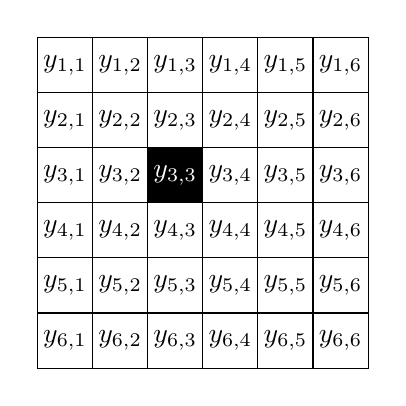
\begin{tikzpicture}

\tikzmath{
	\S = 0.7cm;
}

\tikzset{square matrix/.style={
    matrix of nodes,
    column sep=-\pgflinewidth, row sep=-\pgflinewidth,
    nodes={draw,
      minimum height=#1,
      anchor=center,
      text width=#1,
      align=center,
      inner sep=0pt
    },
  },
  square matrix/.default=\S
}

\matrix[square matrix]
{
$y_{1,1}$ & $y_{1,2}$ & $y_{1,3}$ & $y_{1,4}$ & $y_{1,5}$ & $y_{1,6}$ \\
$y_{2,1}$ & $y_{2,2}$ & $y_{2,3}$ & $y_{2,4}$ & $y_{2,5}$ & $y_{2,6}$ \\
$y_{3,1}$ & $y_{3,2}$ &|[fill=black,text=white]| $y_{3,3}$ & $y_{3,4}$ & $y_{3,5}$ & $y_{3,6}$ \\
$y_{4,1}$ & $y_{4,2}$ & $y_{4,3}$ & $y_{4,4}$ & $y_{4,5}$ & $y_{4,6}$ \\
$y_{5,1}$ & $y_{5,2}$ & $y_{5,3}$ & $y_{5,4}$ & $y_{5,5}$ & $y_{5,6}$ \\
$y_{6,1}$ & $y_{6,2}$ & $y_{6,3}$ & $y_{6,4}$ & $y_{6,5}$ & $y_{6,6}$ \\
};

\end{tikzpicture}

%
% If not, use
%\picplace{5cm}{2cm} % Give the correct figure height and width in cm
%
\caption{If the width of the figure is less than 7.8 cm use the \texttt{sidecapion} command to flush the caption on the left side of the page. If the figure is positioned at the top of the page, align the sidecaption with the top of the figure -- to achieve this you simply need to use the optional argument \texttt{[t]} with the \texttt{sidecaption} command}
\label{fig:exampleca}
\end{figure}
%

\begin{example}[CA with Moore neighborhood and binary states]
\label{ex:simpleca}
Figure \ref{fig:exampleca} shows a simple square 6x6 CA
where the alphabet is $\mathcal{A}=\{ 0, 1 \}$ and the
cells are: $E = \left\{ y_{i,j} : i,j = 1 \dots 6 \right\}$. The neighborhood of cell $y_{3,3}$
is shown, as it is possible to see, it is a Moore neighborhood because all surrounding cells are
included.
\end{example}

\begin{example}[Von Neumann neighborhood]
\label{ex:vnneigh}
With reference to example \ref{ex:simpleca}, we can also see the Van Neumann neighborhood of
cell $y_{4,4}$. In this case, not how only the North, East, South and West surrounding cells
are included.
\end{example}

\begin{important}{Important}
We are going to use always the Moore neighborhood for our analysis, also we will only consider
unit-radius neighborhoods ($r=1$). So, from now on we will always implicitely consider:
$B\left( y_{i,j} \right) = B^\text{M}_1\left( y_{i,j} \right)$.
\end{important}

The last information we need to add about CA, before we can start playing with them, is time.
CA are dynamic objects, they change in time. Before we talk about how they change, we need to
understand how time is modeled in a CA. In mathematical jargon, we say that time is 
\textit{discrete} or, in engineering terms, \textit{slotted}. Normally time is always seen as a
\textit{continuous} entity: a real number: $t \in \mathbb{R}$; thanks to this extreme level of
granularity, we can identify a time instant using a decimal number with a level of precision as high
as we wish (number of decimal digits).
A date and a time can always be converted into a single real number,
the 5\textsuperscript{th} of June 2019 15:55:35 is a date and time that can be converted into seconds
(after Christ's birth), in this case that number would (approximately) be:
\begin{align*}
2019 y + 6 m + 5 d + 15 h + 55 m + 35 s &=\\
2019 \cdot 12 m + 6 \cdot 30 d + 5 \cdot 24 h + 15 \cdot 60 m + 55 \cdot 60 s + 35 s &=\\
2019 \cdot 12 \cdot 30 d + 6 \cdot 30 \cdot 24 h + 5 \cdot 24 \cdot 60 m +
    15 \cdot 60 \cdot 60 s + 3300 s + 35 s &=\\
2019 \cdot 12 \cdot 30 \cdot 24 h + 6 \cdot 30 \cdot 24 \cdot 60 m
    + 5 \cdot 24 \cdot 60 \cdot 60 s +
    54000 s + 3335 s &=\\
2019 \cdot 12 \cdot 30 \cdot 24 \cdot 60 m + 6 \cdot 30 \cdot 24 \cdot 60 \cdot 60 s
    + 432000 s + 57335 s &=\\
2019 \cdot 12 \cdot 30 \cdot 24 \cdot 60 \cdot 60 s + 15552000 s + 489335 s &=\\
62798976000 s + 16041335 s &= 62815017335 s
\end{align*}
Of course, that is not the exact number, as we have simplified things by considering one month always
to be 30 days. But you get the idea. That final number represents
the exact moment when I blew my candels during my birthday this year. And if I had had a stopwatch, I could
even count the milliseconds and add them as a decimal part. This (continuous) vision of time is ideal
when we want to be able to pinpoint an exact instant.

However we don't always need that much precision, sometimes we just want to count events. For example,
we want to count the number of participants at the opening ceremony of every Olympic Game so far.
Those are single events in time, it does not matter to have the precise date and time, we could
just use a natural number to indicate which edition of the Games we are considering. In this example,
we chose to describe time as a \textit{discrete} variable, which means that $t \in \mathbb{N}$.\\

So, now that we have understood time, we can move forward and talk about \textit{evolution}.
CA are very dynamic systems, but so far we have only seen a bunch of cells, each one with a state and
that's it. Well the whole idea is that the CA will change (evolve) in time. This evolution is
represented by a change in the state of every single cell. But how does it happen?

In a CA, time is discrete. The type of events that will make time change depends on the specific model,
hence, at the moment, we just consider time as a meaningless natural number $t \in \mathbb{N}$
that indexes the $t$-th cycle of evolution; once we get to work on a specific model, each cycle will
actually represent something.
At every cycle $t$,
the state of every cell might be different or the same from cycle $t-1$, and this mutation will make
the CA change \textit{configuration} every time.

\begin{definition}[CA configuration]
The \textit{configuration} of a CA at time $t \in \mathbb{N}$, is the set of states of all cells
in the CA at that time: $x_t = \left\{ y^{(t)}_{i,j} \in E \right\}$, where
$y^{(t)}_{i,j}$ represents the state of cell $y_{i,j}$ at time $t$.
\end{definition}

And here comes the final question: how does the state of a cell change? This is where its
neighborhood comes into play.
What is the purpose of a cell's neighborhood? As we mentioned before in definition \ref{def:neigh},
the neighborhood of $y_{i,j}$ contains all the cells $y_{h,k}$ to which $y_{i,j}$ is connected to.
In a CA, the connections are extremely important because the state of one cell will change depending
on the state of every neighbor cell. That's it: the future state of a cell is (also, not only)
determined by the state of its neighbor cells.

\begin{proposition}[Cell state change]
\label{prop:statechange}
In a CA, the state of a cell $y_{i,j} \in E$ in the next cycle $t+1$ depends on 3 factors:
\begin{enumerate}
\item The current cell's state: $y^{(t)}_{i,j}$.
\item The current state of all its neighbor cells: $y^{(t)}_{h,k} \in B\left( y_{i,j} \right)$.
\item Other conditions, specific to the model.
\end{enumerate}
\end{proposition}

When we take proposition \ref{prop:statechange} and write it in mathematical terms, we
get the following:

\begin{definition}[State transition function]
\label{def:statetransf}
Given a CA, we introduce the \textit{cell state transition function}:
\begin{equation}
y^{(t+1)}_{i,j} = f \left[ y^{(t)}_{i,j}, 
    \left\{ y^{(t)}_{h,k} : y_{h,k} \in B\left( y_{i,j} \right) \right\}, \cdot \right]
\end{equation}
Function $f$ defines how the three factors in proposition \ref{prop:statechange}
are used to compute the next state of a cell. $f$ is different in every model.
\end{definition}

Enough with theory, let's make an example.

\begin{example}[Evolution of the LED grid CA]
\label{ex:stateled3}
Recalling example \ref{ex:stateled2}, let's see how we can define a transition function for our
1x3 LED grid to show how this CA can evolve in time. In order to design $f$, we need to define
a neighborhood for each cell. In this simple example, we set every cell to have only one neighbor:
the cell to its right. This means that: $B\left( y_{1,1} \right) = \left\{ y_{1,2} \right\}$,
$B\left( y_{1,2} \right) = \left\{ y_{1,3} \right\}$ and 
$B\left( y_{1,3} \right) = \left\{ y_{1,1} \right\}$ (as you can see, the last cell's
neighbor is the first cell).
Recall that $f$ needs the current cell
and all its neighbors to work, so its input will always be two cells.
In this example, we decide to design $f$ as follows:
\begin{equation*}
f \left( y, y^\prime \right) =
  \begin{cases}
    0       & \quad y = 0 \wedge y^\prime = 0\\
    1       & \quad y = 0 \wedge y^\prime = 1\\
    1       & \quad y = 1 \wedge y^\prime = 1\\
    0       & \quad y = 1 \wedge y^\prime = 0
  \end{cases}
\end{equation*}
Where, $y \in E$ is the current cell and $y^\prime \in E$ its neighbor.
Function $f$ will set the next state in every cell at every cycle $t \in \mathbb{N}$. If we have a look
at its definition, we see that it works in a simple way: the current cell will assume, in $t+1$, the state
of its neighbor at cycle $t$. In fact, the above definition can be simplified as:
\begin{equation*}
f \left( y, y^\prime \right) = y^\prime
\end{equation*}
Let's now have a look at how the CA changes according to $f$ so defined.
We need to set an initial configuration for the CA at $t=0$; this cycle is special as it is the
\textit{initial cycle}. Let's indicate with 
$x_t = \left[ y^{(t)}_{1,1}, y^{(t)}_{1,2}, y^{(t)}_{1,3} \right]$ the configuration of the CA
at cycle $t$. If we start from this initial condition:
$x_0 = (0,0,0)$, how will the CA evolve? The next state of the first cell, is the state of the second
cell, which is $0$. So is the next state of the second cell and the third: $x_1 = (0,0,0)$. If we try
to compute the configuration for the next cycle, we will get the same result. This CA, when given
such an initial condition, will not evolve at all, it will remain the same.

Let's try another initial condition: $x_0 = (0,1,0)$. In this scenario, the middle LED is on.
If we compute the next configuration, we get: $x_1 = (1,0,0)$. If we move on to the next cycle:
$x_2 = (0,0,1)$. And, the next cycle: $x_3 = (0,1,0)$, the CA goes back to its initial condition
to start over again. In this specific scenario, we would see the LEDs creating a cycling linear pattern.
\end{example}

\begin{example}[Another flavor of the LED grid CA]
\label{ex:stateled4}
We keep the same setting of example \ref{ex:stateled3} and change one thing: the transition function
as follows:
\begin{equation*}
f \left( y, y^\prime \right) =
  \begin{cases}
    0       & \quad y = 0 \wedge y^\prime = 0\\
    1       & \quad \text{otherwise}
  \end{cases}
\end{equation*}
Now the CA will work differently from the one in the previous example. Here, in fact, the rule is
that a LED will be stay off only if it is currently off and so is its neighbor. With this
new $f$, let's see what happens when we use the same initial conditions in example \ref{ex:stateled3}.

It is quite trivial to see that the null initial state $x_0 = (0,0,0)$ will cause the CA to behave
like the previous one: no evolution, all LEDs will always remain off.

So let's try the other initial condition: $x_0 = (0,1,0)$. In the first cycle: $x_1 = (1,1,0)$.
In the second cycle, we have: $x_2 = (1,1,1)$. From now on, the CA will remain the same, keeping
configuration $x_t = x_2, \forall t > 2$. So, in this particular CA, when we start with one LED on,
all LEDs will eventually become on.
\end{example}

\begin{problem}
Check that, in example \ref{ex:stateled4}, all initial configurations different from $(0,0,0)$ will
make the CA evolve towards state $(1,1,1)$.
\end{problem}

Thanks to examples \ref{ex:stateled3} and \ref{ex:stateled4}, we have learnt a few important
aspects of CA which are worth mentioning.

\begin{theorem}[CA evolution and initial conditions]
\label{theo:evinitcond}
Given a CA, its evolution depends on the initial condition $x_0$.
\begin{proof}
In both examples \ref{ex:stateled3} and \ref{ex:stateled4}, we could see how the same CA behaved
differently when started from two different initial conditions.
\end{proof}
\end{theorem}

In the example we saw before, we could see how a CA starts from an initial condition 
to reach, possibly, some sort of destination:

\begin{definition}[Final configuration]
\label{def:finalconf}
Given an initial condition/configuration $x_0$, 
it is possible that a CA evolves into a configuration
$x^\ast$ which, once taken, will never be abandoned. If such a configuration exists, we call it
a \textit{final configuration}. When this happens, we write:
$x_0 \overset{f}{\rightarrow} x^\ast$.
We also say that the CA \textit{converges} to $x^\ast$ from $x_0$.
\end{definition}

In example \ref{ex:stateled4}, we could see that any initial configuration with at least one
LED on will lead to all LEDs on. In the specific case, we saw that:
$(0,1,0) \overset{f}{\rightarrow} (1,1,1)$.

\begin{proposition}[Static condition]
When an initial condition $x_0$ causes a CA not to change (not to evolve), we say that
$x_0$ is a \textit{static configuration}.
\end{proposition}

In example \ref{ex:stateled3}, we saw that $(0,0,0)$ is a static configuration.

\begin{proposition}[Recurrent condition]
When an initial condition $x_0$ causes a CA to change different configurations and, after
$T \in \mathbb{N}$ cycles, take that same initial condition and repeat the cycle, we say
that $x_0$ is a \textit{cyclic (or recurrent) configuration of period $T$}.
\end{proposition}

In example \ref{ex:stateled3}, we saw that $(0,1,0)$ is a cyclic configuration of period 3.

\begin{problem}
Prove that, in example \ref{ex:stateled3}, initial condition $(1,0,1)$ is a cyclic configuration
and calculate its period.
\end{problem}

We now know the essentials about CA, we can start creating some interesting models.


%%%%%%%%%%%%%%%%%%%%
%%%%%%%%%%%%%%%%%%%%
%%
%% Andrea Tino - 2019
%% Programming + Science
%% Opinion model
%%
%%%%%%%%%%%%%%%%%%%%
%%%%%%%%%%%%%%%%%%%%

\section{Building our first CA: Conway's Game of Life}
\label{sec:simpleca}

We want to create our first CA in code, so that we can display the cells and see them changing
state. In this section, we will build the basic architecture of a CA that can be used to build any
CA in future. For this, we are going to use the latest web technologies to create web sites and
web applications in the browser: Javascript, HTML and CSS.

\subsection{Creating the basic project structure}
In our PC, let's create a directory (anywhere you want, on your Desktop maybe?) and give it
a cool name like: \texttt{cellautom}. Inside this new directory, do the following:

\begin{enumerate}
\item Create a file and name it: \texttt{index.html}.
\item Create a file and name it: \texttt{ca.js}.
\item Create one last file and name it: \texttt{style.css}.
\end{enumerate}

These three files represent the basic organization of our visual CA we are going to develop.
Table \ref{tab:files} offers a good overview of what they are needed for.

%
% Table
%
\begin{table}[!t]
\centering
\caption{List of files in our project folder.}
\label{tab:files}
%
% Follow this input for your own table layout
%
\begin{tabular}{p{0.2\textwidth}p{0.2\textwidth}p{0.5\textwidth}}
\hline\noalign{\smallskip}
File & Type & Description \\
\noalign{\smallskip}\svhline\noalign{\smallskip}
\texttt{index.html} & Web page & This is the web page that will display the CA and its evolution.\\
\texttt{ca.js} & Javascript code file  & This file will contain the Javascript
code that will make the CA appear and evolve.\\
\texttt{style.css} & CSS Stylesheet & The stylesheet we will use to apply colors, fonts 
    and make our CA beautiful.\\
\noalign{\smallskip}\hline\noalign{\smallskip}
\end{tabular}
\end{table}
%

% Figure
%
\begin{figure}[b]
\sidecaption
% tikz diagram
%
% Forest Diagram
%

\begin{forest}
    for tree={
      font=\ttfamily,
      grow'=0,
      child anchor=west,
      parent anchor=south,
      anchor=west,
      calign=first,
      inner xsep=7pt,
      edge path={
        \noexpand\path [draw, \forestoption{edge}]
        (!u.south west) +(7.5pt,0) |- (.child anchor) pic {folder} \forestoption{edge label};
      },
      % style for file node 
      file/.style={edge path={\noexpand\path [draw, \forestoption{edge}]
        (!u.south west) +(7.5pt,0) |- (.child anchor) \forestoption{edge label};},
        inner xsep=2pt,font=\small\ttfamily
                   },
      before typesetting nodes={
        if n=1
          {insert before={[,phantom]}}
          {}
      },
      fit=band,
      before computing xy={l=15pt},
    }  
  [your-computer
    [cellautom
      [index.html,file
      ]
      [ca.js,file
      ]
      [style.css,file
      ]
    ]
  ]
\end{forest}

%
% If not, use
%\picplace{5cm}{2cm} % Give the correct figure height and width in cm
%
\caption{Your project folder should look like this.}
\label{fig:dirstruct1}
\end{figure}
%

\subsection{Defining the barebones}
Time to write the initial code to see something appear on the page once we run it in the browser.
Open file \texttt{index.html} with your favorite editor.

\begin{programcode}{index.html}
Write this code minding casing and spacing.
\begin{codehtml}
<!DOCTYPE html>
<html>
<head>
  <title>My Cellular Automaton</title>
</head>

<body>
  Hello world!
</body>
</html>
\end{codehtml}
\end{programcode}

Save the file and now try to open it in your browser: we have just displayed a text!

\begin{tips}{A first glance at HTML}
The code we just wrote is read by the browser to create a graphical visualization. HTML is used to
create web pages. It is not a \textit{programming language} (it does not tell a computer what to do),
but a \textit{markup language} (it tells a computer what to display and paint on the screen).

A minimal HTML page looks exactly like the one we just wrote.
It is all based on the concept of \textit{tags}. The
first line \texttt{<!DOCTYPE html>} is special and tells the browser that we are using the latest
version of HTML (you should always use this). Then a new tag \texttt{<html>} is opened and is
closed at the end of the file: \texttt{</html>}. An opening tag and a closing tag make a \textit{block}.
Blocks can contain other blocks.

The \texttt{<html>} block must contain, in order, two other blocks:
\texttt{<head>} and \texttt{<body>}. The first block contains the \texttt{<title>}
block for defining the title of the page
(this text is displayed on the browser's top bar). Everything inside \texttt{<head>} will not generate any 
graphics, it only contains information about the page. What's inside \texttt{body} is, on the other hand, 
painted (or, more technically speaking, rendered\footnote{The term \textit{render} is used to indicate
the complex set of operations that a program does in order to visualize something on the screen.})
inside the browser window. As you can see, we only have a piece of 
text\footnote{The \textit{Hello World} is, historically, the first thing one learns
to do when studying and playing with a new language, we had to respect tradition here.}, which
is in fact rendered on a blank, empty page.
\end{tips}

Of course, we don't just want to display text, we want to render a full CA! So, in the same file, replace
that text.

\begin{programcode}{index.html (snippet)}
Remove \texttt{Hello world!} and insert a \texttt{<div>} block instead.
\begin{codehtmlh1}{1}{3}
<body>
  <div id="ca"></div>
</body>
\end{codehtmlh1}
\end{programcode}

A \texttt{<div>} block is used to group things. We are going to write some code that puts some graphics
inside it. Before leaving this file, we need to import inside it the other two files we have created.

\begin{programcode}{index.html (snippet)}
Place these new tags right below block \texttt{<title>}.
\begin{codehtmlh1}{2}{5}
<head>
  <title>My Cellular Automaton</title>
  <script src="ca.js"></script>
  <link rel="stylesheet" href="style.css">
</head>
\end{codehtmlh1}
\end{programcode}

The first new tag we have added is a \texttt{<script>} which instructs the browser to load and run the
Javascript code inside \texttt{ca.js}. The next one is a \texttt{<link>} tag (this one does not have a closing
tag\footnote{Some tags do not have a closing tag and some do. There is not a rule, you just have
to memorize.})
and tells the browser to load the styles defined inside \texttt{style.css}. As of now, if you refresh the
page in the browser, you will just see a blank page (not for long!).

\subsection{Creating the grid}
For now, we are done with \texttt{index.html}; the next step is to write the code to render the automaton
in our page. To do this, let's open \texttt{ca.js} and insert the first lines of code.

\begin{programcode}{ca.js}
These first lines of Javascript code create our \textit{module}.
\begin{code}
(function(){
  // This is a module
})();
\end{code}
\end{programcode}

We have just created a \textit{module}, let's try to understand a bit more about them.

\begin{tips}{Javascript modules}
Javascript language does not have an intrinsic concept of module, this is something programmers create in
different ways. A \textit{module} is a programming structure encapsulating some code that is isolated
from other codes running in the page.

It is a very generic definition because there is really not much more about it. For now, everytime
we write some code that needs to run in the page, we will wrap it inside a module like shown before,
this is a standard procedure to make sure other Javascript codes on the page, in future, do not
affect our code. Modules also guarantee that our code does not have any side
effects on other scripts running on the same page.
\end{tips}

We have imported \texttt{ca.js} inside \texttt{index.html}, so when we refresh the page the module
we wrote will run. However, since there is really no code inside the module (just a comment),
nothing will happen. Our objective here is to render a grid of cells which will be our automaton,
to achieve this, let's start by defining a few constants:

\begin{programcode}{ca.js}
Define the constants we will use at the beginning on the module.
\begin{codeh1}{1}{5}
(function(){
  const rowsnum = 9;
  const colsnum = 9;
  const cellsize = 20; // In px
})();
\end{codeh1}
\end{programcode}

The constants we defined will be used to create an automaton of the size we specify in 
\texttt{rowsnum} and \texttt{colsnum}. Constant \texttt{cellsize} will be used to defined the
width and height of each (square) cell. Moving on, we now want to create the code that renders the grid.

\begin{programcode}{ca.js}
Inside the module, after the constants, add a function and the code to invoke it.
\begin{codeh1}{5}{13}
(function(){
  const rowsnum = 9;
  const colsnum = 9;
  const cellsize = 20; // In px

  function create() {
    // Here the code to create the grid
  }

  window.addEventListener("load", function() {
    create();
  });
})();
\end{codeh1}
\end{programcode}

We have added two things: we have defined function \texttt{create}, and we have added some code in
the module that uses \texttt{window.addEventListener}. This is what happens when we run the page:

\begin{enumerate}
\item The module is executed.
\item Function \texttt{window.addEventListener} is run. This code will register a function (the one
passed as second parameter) and invoke it, once the event specified in the first parameter fires.
\item When the page has finished loading and everything is ready, function \texttt{create} is called.
\end{enumerate}

If we didn't use \texttt{window.addEventListener}, but just executed \texttt{create()}, our
application might fail sometimes. This code guarantees that we start doing things only when
the page is fully loaded; we need this guard and it is good practice to always write it.

\begin{programcode}{ca.js (snippet)}
Add a new function after function \texttt{create} inside the module.
\begin{codeh1}{4}{8}
function create() {
  // Here the code to create the grid
}

function getContainer() {
  return document.getElementById("ca");
}
\end{codeh1}
\end{programcode}

Function \texttt{getContainer} is going to be important for us later. This function simply
uses \texttt{document.getElementById} to retrieve the \texttt{<div>} we added before in
\texttt{index.html} (we do this by using the \texttt{id} property on the tag).
At this point, we are ready to fill function
\texttt{create} with the code which renders the grid inside the page.

\begin{programcode}{ca.js (snippet)}
Focusing on function \texttt{create}, remove the comment and add this code instead.
\begin{codeh1}{1}{16}
function create() {
  let container = getContainer();
  container.style.width = (colsnum * cellsize + colsnum) + "px";

  for (let i = 1; i <= rowsnum; i++) {
    for (let j = 1; j <= colsnum; j++) {
      let cell = document.createElement("div");
      cell.id = i + ":" + j;
      cell.classList.add("cell");
      cell.style.width = cellsize + "px";
      cell.style.height = cellsize + "px";

      container.appendChild(cell);
    }
  }
}
\end{codeh1}
\end{programcode}

The code above does a few things. In the first lines, we get a reference to the CA container
(the \texttt{<div>} in the page), and set its width according to the size we specified in the
constants. Later on, we create a row-by-column scanning by using one loop nested into the other.
The outer loop will be used to set the current row, the inner loop to set the column. The code
inside the two loops will be executed $\text{rowsnum} \times \text{colsnum}$ times
(for each cell to create).

The code inside the loops first creates a \texttt{<div>} block, then assigns it an id (very
important step, so that we can reference each cell later
by using \texttt{document.getElementById}), adds a style class to it and defines its width and height.
The last command invokes \texttt{appendChild} on the container: this will make the cell appear
inside the container.\\

Try to refresh the page! What can you see? Not really what we were hoping right? Well, the fact that
we cannot see mush does not mean that the page is empty. Let's have a look by inspecting the page
using the F12 tool. If we do so, the tool will display, under the \textit{Elements} tab, the
content of the page: our \texttt{<div>}s are there, it's just that the browser is not rendering
them on the page the way we want. The problem is styling, we must properly style the elements we
have created by using some CSS.

\begin{programcode}{style.css}
Insert this code in \texttt{style.css}.
\begin{codecss}
body {
  margin: 10x;
  padding: 10px;
}

#ca {
  background-color: #000;
  display: flex;
  flex-wrap: wrap;
  padding-left: 1px;
  padding-top: 1px;
}

.cell {
  border: none;
  background-color: #fff;
  margin-right: 1px;
  margin-bottom: 1px;
  flex: 0 0 auto;
}
\end{codecss}
\end{programcode}

We have filled the stylesheet with 3 sets of rules. The first set is for the \texttt{<body>} element
and just defines a 10 pixel spacing between the borders and the content of the whole page.
The second targets
all elements with \texttt{id="ca"} (which is our container): we set the background to black and
make sure all contained cells are wrapped by using \texttt{display: flex} and \texttt{flex-wrap: wrap}.
These last two properties are used to make the cell container a wrapping container. The cells will be
arranged inside the container top-down and left to right. They start from the top-left corner and every
cell is added on the left. When the right border of the container is reached, the next cell will be placed
down on the left to fill a second row, and so on. This behavior is possible thanks to the flex system
we have just used.

If you try to refresh the page now, you will see the grid!

\begin{trailer}{Media content}
You can find the code for this project up to this point in folder \texttt{v2.3}.
\end{trailer}

\begin{problem}
\label{prob:changecasize}
Change the size of the CA/grid by setting it to different dimensions. Also try to make rectangular
automata, not just square grids.
\end{problem}

\subsection{Coding the evolution logic}
We have succeeded rendering the grid, but at the moment our CA doesn't do much, it does nothing!
The key feature of CA is, as we learned at the beginning of this chapter, their ability to
\textit{evolve}. We need to write down that
logic\footnote{Developers use the term \textit{logic} a lot to refer to a behavior that they need
to develop for an application. In our case, we need to code the behavior of evolution in the CA,
so that it can change configuration during every cycle. You can replace the word
\textit{behavior} with \textit{logic}, as many among software engineers and programmers like to
use the latter in their everyday jargon.}.

But what kind of CA are we going to build? What is the state going to be? How about the neighborhood? We
need to define all these properties. The CA we are going to build is a simple and very famour one called:
\textit{Conway's Game of Life} (CGL) \cite{wolfram-ca}.
This CA has the following characteristics:

\begin{itemize}
\item The set of states (alphabet) is: $\mathcal{A} = \{ 0, 1 \}$, where $0$ means "off" (inactive, dead) and
$1$ means "on" (active, alive).
\item Each cell has a Moore neighborhood (recall definition \ref{def:neighmoore} and example \ref{ex:simpleca}).
\item The CA describes pixels in a screen. When a pixel (cell) is on, it turns black; when it's off, it
turns white. 
\end{itemize}

This CA was the first ever published in the history of Mathematics, and it has very interesting properties.

\subsubsection{Setting the initial state}
In CA, it is crucial that we are able to set the initial condition (remember what we talked about in
theorem \ref{theo:evinitcond}). To do so, let's add this code.

\begin{programcode}{ca.js (snippet)}
Insert this constant in \texttt{ca.js} right after the existing contants at the beginning of the module.
\begin{codeh1}{1}{3}
const cellsize = 20; // In px
const initConfig = ["2:2", "4:7", "7:4", "5:5", "3:8"];
\end{codeh1}
\end{programcode}

The line we have added defines a constant which will hold the array of cell identifiers with an initial state
of $1$ in the CA. The code we have at the moment simply creates the cells and nothing more;
as soon as we finish rendering the grid, we must set the initial state.

\begin{programcode}{ca.js (snippet)}
Add this function just below function \texttt{create} inside the module.
\begin{code}
function initializeGrid() {
  for (let i = 1; i <= rowsnum; i++) {
    for (let j = 1; j <= colsnum; j++) {
      if (initConfig.indexOf(i + ":" + j) >= 0) {
        set(i, j, 1);
      } else {
        set(i, j, 0);
      }
    }
  }
}
\end{code}
\end{programcode}

We are going to invoke \texttt{initializeGrid} right after the grid is rendered. As you can see, we traverse
all cells by scanning them row by column as we did before. Inside both loops, we invoke function \texttt{set}
(this function does not exist yet, we will write it in a moment) which will configure the cell state to either
$0$ or $1$ depending on whether the cell identifier is in the \texttt{initConfig} list or not. This will allow us
to set the initial configuration of the CA.

\begin{important}{Bottom-up vs. top-down programming}
We cannot execute the code at this time yet because we still need to write function \texttt{set}.
This approach we have chosen now is a bit different from before. Previously, if, say, function $B$ had to
be called inside function $A$, we would write function $B$ first, and then write down function $A$. Now we are
doing the opposite. The first approach is called \textit{bottom-up programming}
as we build from the foundations and then add on top.
The latter is called \textit{top-down programming} because we start from the higher levels, then moving down
writing what's needed.

The good thing of bottom-up coding is that it's possible to gradually test and run the code at 
every step, but the final algorithm takes
shape later. On the other end, top-down programming is cumbersome, because we cannot test our progress until
all the layers have been built, but the code takes the final shape from the very beginning.
\end{important}

We have written the function responsible for initializing the CA, but we have only defined it, no place in code
is invoking it. We need to invoke it, where? As we mentioned, this phase must occur right after the grid is
rendered; who renders the grid? That would be function \texttt{create}, and who calls that function? If you
scroll down in \texttt{ca.js}, you see that, at the end of the module, the module itself calls it!

\begin{programcode}{ca.js (snippet)}
Invoke function \texttt{initializeGrid} right after calling \texttt{create}.
\begin{codeh1}{2}{4}
window.addEventListener("load", function(){
  create();
  initializeGrid();
});
\end{codeh1}
\end{programcode}

At this point we have almost everything, as soon as the page starts, the grid is created and then
\texttt{initializeGrid} will be called to set the initial state. However that function is trying to
call \texttt{set}, which is another function we still need to define. The purpose of function
\texttt{set(row, column, value)} will be to set the value of the cell at position
$(\text{row}, \text{column})$ to the value in parameter \texttt{value}: $0$ means off and $1$ means on.

\begin{programcode}{ca.js (snippet)}
Add this function right below \texttt{initializeGrid}.
\begin{code}
function set(i, j, value) {
  let cell = getCell(i, j);
  cell.setAttribute("data-value", value);
}
\end{code}
\end{programcode}

The function will first try to get the HTML element of the cell, and then it will try to set attribute
\texttt{data-value} to that. As you can see, here as well we are doing top-down programming because
function \texttt{getCell} does not yet exist, we need to write it.

\begin{programcode}{ca.js (snippet)}
Add this function right above \texttt{set}.
\begin{code}
function getCell(i, j) {
  return document.getElementById(i + ":" + j);
}
\end{code}
\end{programcode}

When we created the grid, we set an identifier to every cell element. Function \texttt{document.getElementById}
is present in every browser and it returns the first HTML element whose \texttt{id} corresponds to the one
provided as input. At this point it seems like everything is done, so try and refresh the page; unfortunately
you will not see anything different. Did we make any mistake? Let's try to see.

\begin{enumerate}
\item Open the browser and refresh the page. You should see the grid.
\item Open the F12 tools and navigate to the \textit{Elements} panel.
\item Expand the \texttt{<body>} tag. Also expand the \texttt{<div id="ca" ...>} tag.
\end{enumerate}

You should, at this point, see the list of \texttt{<div>} tags that represent the cells. See how, in correspondance
of the IDs in array \texttt{initConfig}, the tag shows \texttt{data-value="1"} (\texttt{data-value="0"}
otherwise). So our logic is actually working. The actual problem is the styling. We want the cells marked with
\texttt{data-value="1"} to appear as black, and not white. So let's head to \texttt{style.css} and make some
modifications.

\begin{programcode}{style.css (snippet)}
Add this code at the bottom of the file.
\begin{codecss}
.cell[data-value="1"] {
  background-color: #000;
}
\end{codecss}
\end{programcode}

Make sure you always save. The code we just added instructs the browser to apply a black background color
to our cells when their HTML elements have attribute \texttt{data-value} set to \texttt{1}.
Now our code is finished and we can refresh the page to see our CA getting an initial
condition.

\begin{problem}
\label{prob:changeinit}
Change the initial condition of the grid. Set to \textit{on} only the following
cells: $(3,1)$, $(1,3)$ and $(4,4)$.
\end{problem}

\subsubsection{Building the UI}
At this point we have succeeded setting the initial condition. This means that we can configure the CA however
we want by just changing array \texttt{initConfig} at the beginning of the module. Our final goal is to
make the CA evolve and see it as it changes. We need to build a \textit{User Interface} (or simply: \textit{UI})
that gives us the ability to:

\begin{enumerate}
\item Render the CA in its next configurartion. We can accomplish this with a button: every time we
click this button, the CA will shift to its next configuration from the current one.
\item Visualize what iteration we are in. We can create a piece of text that displays a number
representing the index of the current configuration (discrete time).
\end{enumerate}

So we basically need to create 2
\textit{controls}\footnote{A web page, or more generally, a user interface in every application or app, is made
of different things: buttons, texts, text boxes, input fields and so on. Each one of them is a piece of the UI,
one common way to refer to them is by using the word: \textit{control} in design jargon.}: one button and
one text label. We want to display them at the bottom of the grid, on the left.

\begin{programcode}{index.html (snippet)}
Add a new \texttt{<div>} block right after the one containing the CA.
\begin{codehtmlh1}{2}{5}
<body>
  <div id="ca"></div>
  <div class="controls">
  </div>
</body>
\end{codehtmlh1}
\end{programcode}

The new \texttt{<div>} we just added will be the container for our button and text label. Next step
is adding them inside their container.

\begin{programcode}{index.html (snippet)}
Place these new lines inside the \texttt{<div>} block we added a moment ago.
\begin{codehtmlh1}{1}{4}
<div class="controls">
  <button id="buttonNext">Next</button>
  <span id="cycleText"></span>
</div>
\end{codehtmlh1}
\end{programcode}

Tag \texttt{<button>} creates, as you probably already figured out, a button. While tag \texttt{<span>}
is used to show text. If you go ahead and refresh the page, you will see the button, but no
label next to it. That is because we need to put some text inside it. Since the text in the label
must show the current CA's iteration, we need to track time.

\begin{programcode}{ca.js (snippet)}
Create a variable in the module right after constant \texttt{initConfig} (add spaces before and after to
have a nice code formatting by separating constants, variables and functions in the module).
\begin{codeh1}{3}{5}
const cellsize = 20; // In px
const initConfig = ["3:4", "3:5", "4:3", "4:4", "5:4"];

let t = 0; // Cycles (time)

function create() {
\end{codeh1}
\end{programcode}

Variable \texttt{t} will keep track of time by storing the current CA's iteration. As you can see, when the
module starts, its initial value is set to \texttt{0}, because the initial configuration is cycle 0!
Now we need to show the value of \texttt{t} in the label we just created. To do this, we create a function
which will update the label text:

\begin{programcode}{ca.js (snippet)}
Add this function in the last part of the module.
\begin{codeh1}{0}{5}
function updateCycleText() {
  let text = document.getElementById("cycleText");
  text.textContent = "cycle " + t;
}

window.addEventListener("load", function () {
\end{codeh1}
\end{programcode}

As you can see, function \texttt{updateCycleText} will first locate the label in our page by using
\texttt{document.getElementById} and ID \texttt{"cycleText"} we placed on that element; so that later
we can access the element's \texttt{textContent} and set it to the value we want. We will invoke
this function everytime the CA moves to the next configuration but also when the CA is first created.
This last part we can actually do now.

\begin{programcode}{ca.js (snippet)}
Invoke function \texttt{updateCycleText} right after we call the function to initialize the grid in
the last part of the module.
\begin{codeh1}{3}{5}
window.addEventListener("load", function () {
  create();
  initializeGrid();
  updateCycleText();
});
\end{codeh1}
\end{programcode}

If we refresh the page now, we will see the label next to the button showing text: "cycle 0". Of course,
if we press the button, nothing happens because we haven't written anything for that yet, so let's add
the code to react and do something when the button is clicked.

\begin{programcode}{ca.js (snippet)}
Add this function in the module right after function \texttt{initializeGrid}.
\begin{code}
function initializeButton() {
  let button = document.getElementById("buttonNext");
  button.addEventListener("click", function(){
    console.log("You have clicked me!");
  });
}
\end{code}
\end{programcode}

This function will search for the button element in the page and then add a listener for the \texttt{click}
event. It means that the function we pass as second parameter to \texttt{addEventListener} will be executed
every time the button is clicked. At the  moment we will just display a message in the console. We
of course need to call function \texttt{initializeButton} to make this happen, we invoke the function
right after the grid has been initialized.

\begin{programcode}{ca.js (snippet)}
Invoke function \texttt{initializeButton} right after we call the function to initialize the grid in
the last part of the module.
\begin{codeh1}{3}{5}
window.addEventListener("load", function () {
  create();
  initializeGrid();
  initializeButton();
  updateCycleText();
});
\end{codeh1}
\end{programcode}

If you refresh the page, make sure the F12 tools are open and visible on your screen, and click the button:
you will see the message appearing in the console.

\subsubsection{Coding the evolution}
Everything is prepared now. We have the CA initialized and we also have the UI to interact with the CA.
Next step is creating the logic to make the automaton evolve.
This piece of code will be executed when we press the button.

\begin{programcode}{ca.js (snippet)}
In function \texttt{initializeButton}, remove the line of code to print to console, and write these lines
instead.
\begin{codeh1}{3}{6}
function initializeButton() {
  let button = document.getElementById("buttonNext");
  button.addEventListener("click", function(){
    next();
    updateCycleText();
  });
}
\end{codeh1}
\end{programcode}

Every time we click the button we do 2 things:

\begin{enumerate}
\item We first move the CA to the next configuration by using
function \texttt{next} (which does not exist yet, we will write it later).
\item We invoke function \texttt{updateCycleText} to update the time label.
\end{enumerate}

Let's write down function \texttt{next} which is the core of the evolution logic we need to develop.

\begin{programcode}{ca.js (snippet)}
Add these lines after function \texttt{set}.
\begin{code}
function next() {
  // Calculate the values
  // Todo

  // Apply the values
  // Todo

  t++;
}
\end{code}
\end{programcode}

We haven't really written the whole logic. Since function \texttt{next} will need to do a few things, we
have just prepared it by defining the 3 main actions. As you can see, we have basically created 3 phases:

\begin{enumerate}
\item Calculating the new states for each cell.
\item Applying the states.
\item Incrementing (updating) time.
\end{enumerate}

We are going to replace the \texttt{// Todo} comments with actual code, but now we need to explain a few
things about why we have decided to use this approach, why we have defined these 2 phases: 
\textit{calculate} and \textit{apply}. Our strategy is to:

\begin{enumerate}
\item Scan all the cells in the CA (as we did before) and calculate the state for each cell.
The new states will be memorized in a temporary location.
\item In the second phase, we are going to scan again the cells, and we will apply the new states.
\end{enumerate}

Why do we want to scan the cells twice? Can't we just scan the cells one time and apply each new state
right after calculating it? The answer is no, because otherwise we would calculate the CA's new configuration
in an undesired way. Look at figure \ref{fig:updatecainc},
the diagram shows what happens if we do not use the double
scanning and the problem of polluting the grid. For this reason we need to scan the cells twice. This is because
our CA is going to be an \textit{immediate CA}, it means that all the cells update at the same time
as shown in figure \ref{fig:updatecaimm}.
With the other
approach, we would otherwise have an \textit{incremental CA}, where every new configuration of a cell depends on the
newly updated value of the neighbors. Incremental CA are not wrong automata,
they are just different. In this chapter,
however, we want to use immediate CA!

% Figure
%
\begin{figure}[b]
\sidecaption
% tikz diagram
%
% Tikz Diagram
%

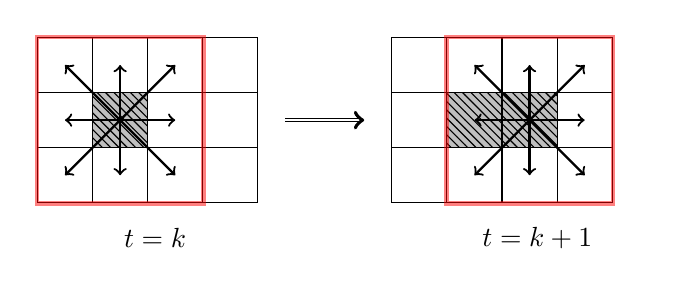
\begin{tikzpicture}

\tikzmath{
	\S = 0.7cm;
}

\tikzset{square matrix/.style={
    matrix of nodes,
    column sep=-\pgflinewidth, row sep=-\pgflinewidth,
    nodes={draw,
      minimum height=#1,
      anchor=center,
      text width=#1,
      align=center,
      inner sep=0pt
    },
  },
  square matrix/.default=\S
}

\matrix[square matrix] (m1) at (0,0)
{
\phantom{} & \phantom{} & \phantom{} & \phantom{} \\
\phantom{} &|[preaction={fill, lightgray}, pattern=north west lines, pattern color=black]| \phantom{} & \phantom{} & \phantom{} \\
\phantom{} & \phantom{} & \phantom{} & \phantom{} \\
};
\draw[opacity=.5, ultra thick, red] (m1-1-1.north west)-|
   (m1-3-3.south east)-|
   (m1-3-1.south west)-|cycle;
\draw [->, thick] (m1-2-2.center) -- (m1-1-1.center);
\draw [->, thick] (m1-2-2.center) -- (m1-1-2.center);
\draw [->, thick] (m1-2-2.center) -- (m1-1-3.center);
\draw [->, thick] (m1-2-2.center) -- (m1-2-1.center);
\draw [->, thick] (m1-2-2.center) -- (m1-2-3.center);
\draw [->, thick] (m1-2-2.center) -- (m1-3-1.center);
\draw [->, thick] (m1-2-2.center) -- (m1-3-2.center);
\draw [->, thick] (m1-2-2.center) -- (m1-3-3.center);

\matrix[square matrix] (m2) at (4.5,0)
{
\phantom{} & \phantom{} & \phantom{} & \phantom{} \\
\phantom{} &|[preaction={fill, lightgray}, pattern=north west lines, pattern color=black]| \phantom{} &|[preaction={fill, lightgray}, pattern=north west lines, pattern color=black]| \phantom{} & \phantom{} \\
\phantom{} & \phantom{} & \phantom{} & \phantom{} \\
};
\draw[opacity=.5, ultra thick, red] (m2-1-2.north west)-|
   (m2-3-4.south east)-|
   (m2-3-2.south west)-|cycle;
\draw [->, thick] (m2-2-3.center) -- (m2-1-2.center);
\draw [->, thick] (m2-2-3.center) -- (m2-1-3.center);
\draw [->, thick] (m2-2-3.center) -- (m2-1-4.center);
\draw [->, thick] (m2-2-3.center) -- (m2-2-2.center);
\draw [->, thick] (m2-2-3.center) -- (m2-2-4.center);
\draw [->, thick] (m2-2-3.center) -- (m2-3-2.center);
\draw [->, thick] (m2-2-3.center) -- (m2-3-3.center);
\draw [->, thick] (m2-2-3.center) -- (m2-3-4.center);

\node[text width=2cm] at (0.7,-1.5) {$t = k$};
\node[text width=2cm] at (5.25,-1.5) {$t = k+1$};

\draw [->, double] (1.75,0) -- (2.75,0);

\end{tikzpicture}

%
% If not, use
%\picplace{5cm}{2cm} % Give the correct figure height and width in cm
%
\caption{An example of incremental CA. As you can see in iteration $t=k$, one cell is updated
with its new state. In the next iteration ($t=k+1$), the next cell is updated, however its state
will be calculated on the new value of the previous.}
\label{fig:updatecainc}
\end{figure}
%

% Figure
%
\begin{figure}[b]
\sidecaption
% tikz diagram
%
% Tikz Diagram
%

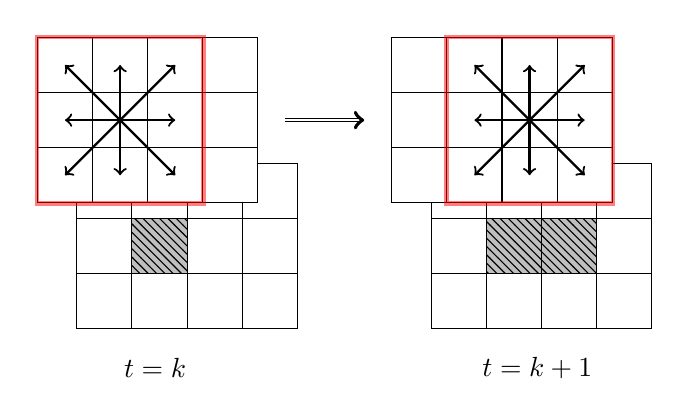
\begin{tikzpicture}

\tikzmath{
	\S = 0.7cm;
}

\tikzset{square matrix/.style={
    matrix of nodes,
    column sep=-\pgflinewidth, row sep=-\pgflinewidth,
    nodes={draw,
      minimum height=#1,
      anchor=center,
      text width=#1,
      align=center,
      inner sep=0pt
    },
  },
  square matrix/.default=\S
}

\matrix[square matrix] (mg1) at (0.5,-1.6)
{
\phantom{} & \phantom{} & \phantom{} & \phantom{} \\
\phantom{} &|[preaction={fill, lightgray}, pattern=north west lines, pattern color=black]| \phantom{} & \phantom{} & \phantom{} \\
\phantom{} & \phantom{} & \phantom{} & \phantom{} \\
};
\matrix[square matrix] (m1) at (0,0)
{
|[fill=white]| \phantom{} &|[fill=white]| \phantom{} &|[fill=white]| \phantom{} &|[fill=white]| \phantom{} \\
|[fill=white]| \phantom{} &|[fill=white]| \phantom{} &|[fill=white]| \phantom{} &|[fill=white]| \phantom{} \\
|[fill=white]| \phantom{} &|[fill=white]| \phantom{} &|[fill=white]| \phantom{} &|[fill=white]| \phantom{} \\
};
\draw[opacity=.5, ultra thick, red] (m1-1-1.north west)-|
   (m1-3-3.south east)-|
   (m1-3-1.south west)-|cycle;
\draw [->, thick] (m1-2-2.center) -- (m1-1-1.center);
\draw [->, thick] (m1-2-2.center) -- (m1-1-2.center);
\draw [->, thick] (m1-2-2.center) -- (m1-1-3.center);
\draw [->, thick] (m1-2-2.center) -- (m1-2-1.center);
\draw [->, thick] (m1-2-2.center) -- (m1-2-3.center);
\draw [->, thick] (m1-2-2.center) -- (m1-3-1.center);
\draw [->, thick] (m1-2-2.center) -- (m1-3-2.center);
\draw [->, thick] (m1-2-2.center) -- (m1-3-3.center);

\matrix[square matrix] (mg2) at (5,-1.6)
{
\phantom{} & \phantom{} & \phantom{} & \phantom{} \\
\phantom{} &|[preaction={fill, lightgray}, pattern=north west lines, pattern color=black]| \phantom{} &|[preaction={fill, lightgray}, pattern=north west lines, pattern color=black]| \phantom{} & \phantom{} \\
\phantom{} & \phantom{} & \phantom{} & \phantom{} \\
};
\matrix[square matrix] (m2) at (4.5,0)
{
|[fill=white]| \phantom{} &|[fill=white]| \phantom{} &|[fill=white]| \phantom{} &|[fill=white]| \phantom{} \\
|[fill=white]| \phantom{} &|[fill=white]| \phantom{} &|[fill=white]| \phantom{} &|[fill=white]| \phantom{} \\
|[fill=white]| \phantom{} &|[fill=white]| \phantom{} &|[fill=white]| \phantom{} &|[fill=white]| \phantom{} \\
};
\draw[opacity=.5, ultra thick, red] (m2-1-2.north west)-|
   (m2-3-4.south east)-|
   (m2-3-2.south west)-|cycle;
\draw [->, thick] (m2-2-3.center) -- (m2-1-2.center);
\draw [->, thick] (m2-2-3.center) -- (m2-1-3.center);
\draw [->, thick] (m2-2-3.center) -- (m2-1-4.center);
\draw [->, thick] (m2-2-3.center) -- (m2-2-2.center);
\draw [->, thick] (m2-2-3.center) -- (m2-2-4.center);
\draw [->, thick] (m2-2-3.center) -- (m2-3-2.center);
\draw [->, thick] (m2-2-3.center) -- (m2-3-3.center);
\draw [->, thick] (m2-2-3.center) -- (m2-3-4.center);

\node[text width=2cm] at (0.7,-3.15) {$t = k$};
\node[text width=2cm] at (5.25,-3.15) {$t = k+1$};

\draw [->, double] (1.75,0) -- (2.75,0);

\end{tikzpicture}

%
% If not, use
%\picplace{5cm}{2cm} % Give the correct figure height and width in cm
%
\caption{An example of immediate CA. By using a temporary CA (a ghost CA) we can update
the state of the cells of the CA without polluting our calculations. After all cells have been scanned, the
ghost CA is used to replace the saved states in the original CA. At the end of the process, the ghost CA is
finally destroyed as no more needed.}
\label{fig:updatecaimm}
\end{figure}
%

In an immediate CA, the states of all cells can actually be updated in parallel. But we are not going to go
that far here (the code for doing this is much more complicated).

We need to talk about one last thing before resuming coding: the \textit{border effect}. We know how to
calculate the next configuration of a CA: we need to compute all the new states of all the cells. And the state
of a cell depends on the state of its neighbors. Normally a cell has 8 neighbors as we explained in definition
\ref{def:neigh}, however the cells on the border have fewer neighbors:

\begin{itemize}
\item If a cell is on the border, it will have 3 neighbors less, for a total of 5.
\item A corner cell loses 5 neighbors, for a total of 3.
\end{itemize}

What do we do with them? There are many approaches: we could have special rules for them when updating their
state for instance.

\begin{example}[Using different rules for border and corner cells]
\label{ex:diffruleset}
Consider a CA where every cell can either be active or inactive, like the LED CA in
example \ref{ex:stateled}; in this automaton we set a transition rule for which 
a cell becomes active only if at least half of its neighbors are active. For a
normal cell that number is 4, but for a border cell or corner cell? We could use a special rule for border
cells and set that number to 2 or 3, and for corner cells we could set that number to 1 or 2.
\end{example}

Using different rules for cells (as suggested in example \ref{ex:diffruleset})
makes the automaton more complex though, and we don't want that.
So we are going to
choose the simplest approach: ignoring border and corner cells. It means that, when computing the next
configuration of a CA, we are not going to update the state of border and corner cells, they will always retain their initial state. Practically speaking, it means that our scanning will exclude border and corner cells
(we will see this in action in code soon). With all this in mind, let's go back to code.

\begin{programcode}{ca.js (snippet)}
Replace the \texttt{// Todo} comments with the following lines.
\begin{codeh2}{2}{8}{9}{15}
function next() {
  // Calculate the values
  for (let i = 2; i <= rowsnum - 1; i++) {
    for (let j = 2; j <= colsnum - 1; j++) {
      // This is the first scan
    }
  }

  // Apply the values
  for (let i = 2; i <= rowsnum - 1; i++) {
    for (let j = 2; j <= colsnum - 1; j++) {
      // This is the second scan
    }
  }

  t++;
}
\end{codeh2}
\end{programcode}

The scanning blocks here are different from those we wrote inside function \texttt{create}.
Look at the indices in the \texttt{for} loops: this time they start from
$2$ not $1$. And they finish with $rowsnum - 1$ and $colsnum - 1$ instead of $rowsnum$ and $colsnum$.
When we do this, we are effectively excluding from the scan all border and corner cells.

We are now ready to start calculating the next state of every cell, however we don't know what
transition rule to follow.

\begin{definition}[State transition rules in Conway's Game of Life]
\label{def:cglrules}
In CGL CA, the transition rules are the following:
\begin{enumerate}
\item Any \textbf{active} cell with fewer than 2 active neighbors becomes \textbf{inactive}.
\item Any \textbf{active} cell with 2 or 3 active neighbors remains \textbf{active}.
\item Any \textbf{active} cell with more than 3 active neighbors becomes \textbf{inactive}.
\item Any \textbf{inactive} cell with exactly 3 active neighbors becomes \textbf{active}.
\item If none of the above rules apply, the cell's state remains \textbf{the same}.
\end{enumerate}
\end{definition}

The first thing we wanna do is translating the rules in definition \ref{def:cglrules} into
actual Javascript code inside our module.

\begin{programcode}{ca.js (snippet)}
Add this code in the module right below function \texttt{next}.
\begin{code}
function calculateState(state, neighSum) {
  if (state === 1 && neighSum < 2) {
    return 0; // Any active cell with fewer than 2 active neighbors becomes inactive
  }
  if (state === 1 && neighSum >= 2 && neighSum <= 3) {
    return 1; // Any active cell with 2 or 3 active neighbors remains active
  }
  if (state === 1 && neighSum > 3) {
    return 0; // Any active cell with more than 3 active neighbors becomes inactive
  }
  if (state === 0 && neighSum === 3) {
    return 1; // Any inactive cell with exactly 3 active neighbors becomes active
  }
  return state; // Otherwise the cell's state remains the same
}
\end{code}
\end{programcode}

Function \texttt{calculateState} implements the 5 rules in the CA as per definition \ref{def:cglrules} and
can be used to calculate the next state of a single cell.
It accepts 2 arguments: \texttt{state} is the cell's current state, and \texttt{neighSum} is the number of
neighbor cells that are active in the current configuration (cycle).
We are going to use this function inside \texttt{next}.

\begin{programcode}{ca.js (snippet)}
Remove comment \texttt{// This is the first scan} from the first scanning double loop and add this
code instead.
\begin{codeh1}{2}{16}
for (let i = 2; i <= rowsnum - 1; i++) {
  for (let j = 2; j <= colsnum - 1; j++) {
    // Cell (i,j)'s state
    let cell = get(i, j);

    // States of cell (i,j)'s neighbors
    let north = get(i - 1, j);
    let south = get(i + 1, j);
    let east = get(i, j + 1);
    let west = get(i, j - 1);
    let northeast = get(i - 1, j + 1);
    let southeast = get(i + 1, j + 1);
    let northwest = get(i - 1, j - 1);
    let southwest = get(i + 1, j - 1);
    let sum = north + south + east + west + northeast + southeast + northwest + southwest;
  }
}
\end{codeh1}
\end{programcode}

% Figure
%
\begin{figure}[b]
\sidecaption
% tikz diagram
%
% Andrea Tino
% 2020
%
% =======================================================================
% Creative Commons Attribution-NonCommercial-ShareAlike 4.0 International
% Public License
% =======================================================================
%

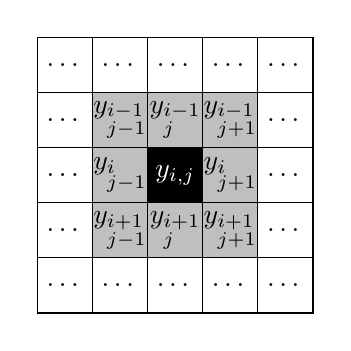
\begin{tikzpicture}

\tikzmath{
	\S = 0.7cm;
}

\tikzset{square matrix/.style={
    matrix of nodes,
    column sep=-\pgflinewidth, row sep=-\pgflinewidth,
    nodes={draw,
      minimum height=#1,
      anchor=center,
      text width=#1,
      align=center,
      inner sep=0pt
    },
  },
  square matrix/.default=\S
}

\matrix[square matrix] (m1) at (0,0)
{
$\dots$ & $\dots$ & $\dots$ & $\dots$ & $\dots$ \\
$\dots$ & |[fill=lightgray]| $y_{\begin{subarray}{l}i-1\\j-1\end{subarray}}$ &|[fill=lightgray]| $y_{\begin{subarray}{l}i-1\\j\end{subarray}}$ &|[fill=lightgray]| $y_{\begin{subarray}{l}i-1\\j+1\end{subarray}}$ & $\dots$ \\
$\dots$ & |[fill=lightgray]| $y_{\begin{subarray}{l}i\\j-1\end{subarray}}$ &|[fill=black,text=white]| $y_{i,j}$ &|[fill=lightgray]| $y_{\begin{subarray}{l}i\\j+1\end{subarray}}$ & $\dots$ \\
$\dots$ & |[fill=lightgray]| $y_{\begin{subarray}{l}i+1\\j-1\end{subarray}}$ &|[fill=lightgray]| $y_{\begin{subarray}{l}i+1\\j\end{subarray}}$ &|[fill=lightgray]| $y_{\begin{subarray}{l}i+1\\j+1\end{subarray}}$ & $\dots$ \\
$\dots$ & $\dots$ & $\dots$ & $\dots$ & $\dots$ \\
};

\end{tikzpicture}

%
% If not, use
%\picplace{5cm}{2cm} % Give the correct figure height and width in cm
%
\caption{A visualization of the neighborhood of a cell in the grid.
A generic cell $(i,j)$ is highlighted in the CA (black)
and its neighborhood is visualized (in grey).
Note how the coordinates of each neighbor cell is expressed relatively
to cell $(i,j)$.}
\label{fig:cellneigh}
\end{figure}
%

The code we have added is needed to collect all the info we need to calculate the next state for every cell.
Recall that in a CA, the new state of a cell is calculated by using:

\begin{itemize}
\item The cell's current state.
\item The current states of the cell's neighbors.
\end{itemize}

We are using top-down programming again by invoking function \texttt{get} (which does not exist yet). This function
will return a cell's current state by passing its row and column number. Apart from that, the code we
just wrote is not dificult to understand: we first get the state of the cell we are scanning, then we get the states
of its neighbors. Figure \ref{fig:cellneigh} provides a good visualization to better understand the code we just
wrote.
We compute 9 variables in total and then we create variable \texttt{sum} which will
contain the number of active neighbors (remember that an active cell has state $1$, $0$ otherwise). In this
code, there is one more thing left to do: calculating the new state and saving it.

\begin{programcode}{ca.js (snippet)}
Always inside the first double loop, add these lines at the end.
\begin{codeh1}{2}{5}
let sum = north + south + east + west + northeast + southeast + northwest + southwest;

// Calculate new state and save it
setTmp(i, j, calculateState(cell, sum));
\end{codeh1}
\end{programcode}

Function \texttt{setTmp} (which we still need to write, yes more top-down programming) will save the new state
for the currently scanned cell in the ghost CA (without polluting the original automaton).
The first two parameters are the row and the column of the cell whose
new state we need to save, the third parameter is the value of the new state, of course we use function
\texttt{calculateState} (which we wrote before) for this task. We have used top-down programming quite often here,
let's write down the code of what's missing: we need to define two functions: \texttt{get} and \texttt{setTmp}.

\begin{programcode}{ca.js (snippet)}
In the module, add this code right below function \texttt{set}.
\begin{code}
function get(i, j) {
  let cell = getCell(i, j);
  let value = cell.getAttribute("data-value") || 0;
  return parseInt(value);
}
\end{code}
\end{programcode}

Function \texttt{get} is quite simple: first we get the \texttt{<div>} element of the cell and then we
extract the value associated with attribute \texttt{data-value}. It is possible that the attribute
is not set on the element, in that case \texttt{getAttribute} would return \texttt{undefined} so we
use operator \texttt{||}.

\begin{tips}{Operator \texttt{||}}
Expression \texttt{a || b} returns \texttt{a} if \texttt{b} is \texttt{undefined}
or \texttt{b} if \texttt{a} is \texttt{undefined}; if both variables have values, then the one on the
left is returned.
\end{tips}

In this case, if there is no state defined for a cell, we assume it is \texttt{0}
(inactive, off).

\begin{programcode}{ca.js (snippet)}
In the module, add these two functions right below function \texttt{get}.
\begin{code}
function setTmp(i, j, value) {
  let cell = getCell(i, j);
  cell.setAttribute("data-tmpvalue", value);
}

function getTmp(i, j) {
  let cell = getCell(i, j);
  return parseInt(cell.getAttribute("data-tmpvalue"));
}
\end{code}
\end{programcode}

The functions we have created, as you can see, look quite similar to functions
\texttt{get} and \texttt{set}. To be specific, we say they have the same
\textit{signature}.

\begin{tips}{Signature of a function}
The signature of a function is the list of its input parameters and the type of returned
value (if any). Consider the following function:
\begin{code}
function greetMe(name, surname) {
  return "Hello " + name + " " + surname;
}
\end{code}
Its signature can be represented as: \texttt{(string, string) => string} as it accepts
two strings and returns another string.
\end{tips}

In fact they do the same thing but on different attributes. Maybe you are getting the
idea now. What we want to do is saving the calculated new state of a cell into a
different attribute called \texttt{data-tmpvalue} during the first scan. In the second scan,
we will then copy the value from \texttt{data-tmpvalue} to \texttt{data-value} on
each cell.

At this point, we have completed writing the first scan. When finishing the first scan,
every cell has memorized its next value in the temporary attribute,
the second scan will apply these values.

\begin{programcode}{ca.js (snippet)}
Remove comment \texttt{// This is the second scan} from the second scanning double loop and add this
code instead.
\begin{codeh1}{2}{5}
for (let i = 2; i <= rowsnum - 1; i++) {
  for (let j = 2; j <= colsnum - 1; j++) {
    set(i, j, getTmp(i, j));
    removeTmpValue(i, j); // Clean up
  }
}
\end{codeh1}
\end{programcode}

The lines we have added complete function \texttt{next}. As every cell is traversed again in the grid,
their new state is read by using \texttt{getTmp} and then applied by using \texttt{set}. After the new
state is applied, we do not need the temporary value anymore, so we destroy it by using function
\texttt{removeTmpValue} which we will write now.

\begin{programcode}{ca.js (snippet)}
In the module, add these lines right below function \texttt{getTmp}.
\begin{code}
function removeTmpValue(i, j) {
  let cell = getCell(i, j);
  cell.removeAttribute("data-tmpvalue");
}
\end{code}
\end{programcode}

Function \texttt{removeTmpValue} is very simple: it first retrieves the \texttt{<div>} element of the cell
(whose coordinates are passed as parameters), and then invokes function \texttt{removeAttribute} which
deletes the \texttt{data-tmpvalue} attribute (effectively clearing the temporary value).

\subsubsection{Final touches}
At this time, you can actually refresh the page and see the CA being rendered and also interact with it.
However we want to spend a short while now making a very few style adjustments to make the page look better.

The first thing we want to do is introducing a little spacing between the grid and the controls below it.

\begin{programcode}{style.css (snippet)}
In the stylesheet, add these lines at the end of the file.
\begin{codecss}
.controls {
  margin-top: 10px;
}
\end{codecss}
\end{programcode}

If you save the file and then refresh the page, you will see
the button and the label now being rendered with a better
spacing from the grid. If you prefer less spacing (or more), just change \texttt{margin-top} to a different
value.

Another thing we want to do is improving the style of the button. We want to make it a plain grey button
with a black text and a better spacing between the text and the borders.

\begin{programcode}{style.css (snippet)}
In the stylesheet, add these lines at the end of the file.
\begin{codecss}
#buttonNext {
  background-color: #ddd;
  color: #000;
  border: none;
  padding: 5px;
}
\end{codecss}
\end{programcode}

By setting \texttt{border: none} we remove the 3D effect on the button which browsers commonly add.
With this style, the button looks simpler and more modern.

If you try to hover with the mouse the button, you will see it's kinda odd that nothing happens. Usually
something signals that the button can be pressed and we are missing that feedback. A link would change to
an underlined text style when hovered, a button typically changes the background to be darker and we want to
achieve that effect. Also, if you click it, the button still has the same style: normally it is good
practice that a button changes style when pressed to give the user some feedback about it. All these
small details might seem minor, but they are quite important.

\begin{programcode}{style.css (snippet)}
In the stylesheet, add these lines at the end of the file.
\begin{codecss}
#buttonNext:hover {
  background-color: #ccc;
}
#buttonNext:active {
  background-color: #bbb;
}
\end{codecss}
\end{programcode}

By using pseudo-classes \texttt{:hover} and \texttt{:active}, we can decide what style the button should
have when the mouse hovers on it, or presses it. If you refresh the page and try to click the button, you
will see the experience has much improved.\\

One last thing, before calling it a fully working automaton, is adding a small piece of code to prevent
errors. What errors? A golden rule that programmers should respect when building configurable applications
is that the configuration parameters are in the allowed range. Why do we bother about this here?
Do we have configuration parameters? Well, turns out that the answer is yes. Look at the beginning
of our module in \texttt{ca.js}: you will see we have created three constants that we use to configure
our automaton. What happens if:

\begin{itemize}
\item The CA is configured to be 2x2?
\item The size of a cell is changed to a negative number?
\end{itemize}

In the first case, the CA would not make much sense because we ignore the border cells remember! A 2x2 CA
is made only of border cells so it would do nothing. Also, a very small CA is not interesting. To have some
kind of observable interesting behavior, we need at least a 9x9 CA. About the second question, well we would
get a very weird rendering. The browser would not accept a negative number for the width or the height of
an element, so we would get unpredictable results. In general, the cells should have a minimum size to be
visible, otherwise the final automaton would look too small. A minimum size of 4 pixels is fair.

\begin{programcode}{ca.js (snippet)}
At the end of the module, add these lines at the indicated position.
\begin{codeh1}{1}{8}
window.addEventListener("load", function () {
  if (rowsnum < 9 || colsnum < 9) {
    throw new Error("The CA must be at least 9x9.");
  }
  if (cellsize < 4) {
    throw new Error("Cells are too small. A cell must be at least 4px!");
  }

  create();
  initializeGrid();
  initializeButton();
  updateCycleText();
});
\end{codeh1}
\end{programcode}

We have just translated in code the conditions we decided a moment ago.

\begin{tips}{Throwing errors}
How can a web application send an error? The proper way of doing it is by using this syntax:
\begin{code}
throw new Error("Your error message here");
\end{code}
When this code is executed, the F12 Javascript console will show an error message with the text
specified inside \texttt{Error} and no more code will be executed.
\end{tips}

If our CA is not configured properly, we emit an error and block the code from running.

\begin{trailer}{Media content}
All the code we have written up to this point can be found under folder \texttt{v2.4}.
\end{trailer}

\subsection{Playing with CGL automaton}
There is a reason if we have decided to build this specific automaton as our first CA! Other than being
the very first one to be published very famous, it has some very interesting properties.
The best way to experience these peculiarities is by playing with them, so try to
solve the following problems all based on the CA we have just built. One recommendation,
set the initial configurations by always avoiding border cells, always try to place
the shapes at the center of the grid (unless asked otherwise).

% Figure
%
\begin{figure}[b]
\sidecaption
% tikz diagram
%
% Tikz Diagram
%

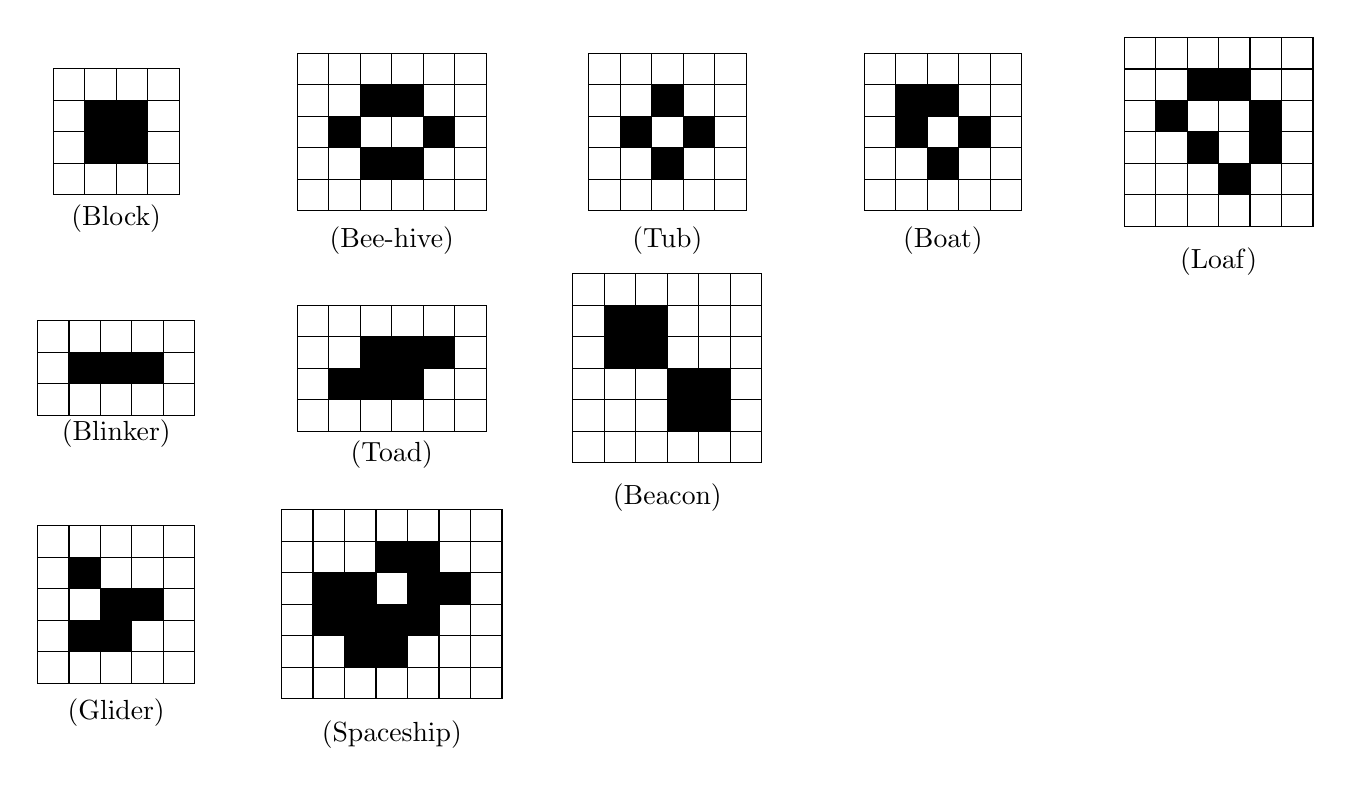
\begin{tikzpicture}

\tikzmath{
	\S = 0.4cm;
  \s = 0.55;
  \X1 = 0;
  \X2 = 3.5;
  \X3 = 7;
  \X4 = 10.5;
  \X5 = 14;
  \Y1 = 0;
  \Y2 = -3;
  \Y3 = -6;
  \tyblock = \Y1 - 4*0.5*\s;
  \tybeehive = \Y1 - 5*0.5*\s;
  \tytub = \Y1 - 5*0.5*\s;
  \tyboat = \Y1 - 5*0.5*\s;
  \tyloaf = \Y1 - 6*0.5*\s;
  \tyblinker = \Y2 - 3*0.5*\s;
  \tytoad = \Y2 - 4*0.5*\s;
  \tybeacon = \Y2 - 6*0.5*\s;
  \tyglider = \Y3 - 5*0.5*\s;
  \tyspaceship = \Y3 - 6*0.5*\s;
}

\tikzset{square matrix/.style={
    matrix of nodes,
    column sep=-\pgflinewidth, row sep=-\pgflinewidth,
    nodes={draw,
      minimum height=#1,
      anchor=center,
      text width=#1,
      align=center,
      inner sep=0pt
    },
  },
  square matrix/.default=\S
}

% Block
\matrix[square matrix] (m1) at (\X1,\Y1)
{
\phantom{} & \phantom{} & \phantom{} & \phantom{} \\
\phantom{} &|[fill=black]| \phantom{} &|[fill=black]| \phantom{} & \phantom{} \\
\phantom{} &|[fill=black]| \phantom{} &|[fill=black]| \phantom{} & \phantom{} \\
\phantom{} & \phantom{} & \phantom{} & \phantom{} \\
};
\node at (\X1,\tyblock) {(Block)};

% Beehive
\matrix[square matrix] (m2) at (\X2,\Y1)
{
\phantom{} & \phantom{} & \phantom{} & \phantom{} & \phantom{} & \phantom{} \\
\phantom{} & \phantom{} &|[fill=black]| \phantom{} &|[fill=black]| \phantom{}& \phantom{} & \phantom{}  \\
\phantom{} &|[fill=black]| \phantom{} & \phantom{} & \phantom{} &|[fill=black]| \phantom{} & \phantom{}  \\
\phantom{} & \phantom{} &|[fill=black]| \phantom{} &|[fill=black]| \phantom{}& \phantom{} & \phantom{}  \\
\phantom{} & \phantom{} & \phantom{} & \phantom{}& \phantom{} & \phantom{}  \\
};
\node at (\X2,\tybeehive) {(Bee-hive)};

% Tub
\matrix[square matrix] (m3) at (\X3,\Y1)
{
\phantom{} & \phantom{} & \phantom{} & \phantom{} & \phantom{} \\
\phantom{} & \phantom{} &|[fill=black]| \phantom{} & \phantom{} & \phantom{} \\
\phantom{} &|[fill=black]| \phantom{} & \phantom{} &|[fill=black]| \phantom{} & \phantom{} \\
\phantom{} & \phantom{} &|[fill=black]| \phantom{} & \phantom{} & \phantom{} \\
\phantom{} & \phantom{} & \phantom{} & \phantom{} & \phantom{} \\
};
\node at (\X3,\tytub) {(Tub)};

% Boat
\matrix[square matrix] (m31) at (\X4,\Y1)
{
\phantom{} & \phantom{} & \phantom{} & \phantom{} & \phantom{} \\
\phantom{} &|[fill=black]| \phantom{} &|[fill=black]| \phantom{} & \phantom{} & \phantom{} \\
\phantom{} &|[fill=black]| \phantom{} & \phantom{} &|[fill=black]| \phantom{} & \phantom{} \\
\phantom{} & \phantom{} &|[fill=black]| \phantom{} & \phantom{} & \phantom{} \\
\phantom{} & \phantom{} & \phantom{} & \phantom{} & \phantom{} \\
};
\node at (\X4,\tyboat) {(Boat)};

% Loaf
\matrix[square matrix] (m32) at (\X5,\Y1)
{
\phantom{} & \phantom{} & \phantom{} & \phantom{} & \phantom{} & \phantom{} \\
\phantom{} & \phantom{} &|[fill=black]| \phantom{} &|[fill=black]| \phantom{} & \phantom{} & \phantom{} \\
\phantom{} &|[fill=black]| \phantom{} & \phantom{} & \phantom{} &|[fill=black]| \phantom{} & \phantom{} \\
\phantom{} & \phantom{} &|[fill=black]| \phantom{} & \phantom{} &|[fill=black]| \phantom{} & \phantom{} \\
\phantom{} & \phantom{} & \phantom{} &|[fill=black]| \phantom{} & \phantom{} & \phantom{} \\
\phantom{} & \phantom{} & \phantom{} & \phantom{} & \phantom{} & \phantom{} \\
};
\node at (\X5,\tyloaf) {(Loaf)};

% Blinker
\matrix[square matrix] (m4) at (\X1,\Y2)
{
\phantom{} & \phantom{} & \phantom{} & \phantom{} & \phantom{} \\
\phantom{} &|[fill=black]| \phantom{} &|[fill=black]| \phantom{} &|[fill=black]| \phantom{} & \phantom{} \\
\phantom{} & \phantom{} & \phantom{} & \phantom{} & \phantom{} \\
};
\node at (\X1,\tyblinker) {(Blinker)};

% Toad
\matrix[square matrix] (m5) at (\X2,\Y2)
{
\phantom{} & \phantom{} & \phantom{} & \phantom{} & \phantom{} & \phantom{} \\
\phantom{} & \phantom{} &|[fill=black]| \phantom{} &|[fill=black]| \phantom{} &|[fill=black]| \phantom{} & \phantom{} \\
\phantom{} &|[fill=black]| \phantom{} &|[fill=black]| \phantom{} &|[fill=black]| \phantom{} & \phantom{} & \phantom{} \\
\phantom{} & \phantom{} & \phantom{} & \phantom{} & \phantom{} & \phantom{} \\
};
\node at (\X2,\tytoad) {(Toad)};

% Beacon
\matrix[square matrix] (m6) at (\X3,\Y2)
{
\phantom{} & \phantom{} & \phantom{} & \phantom{} & \phantom{} & \phantom{} \\
\phantom{} &|[fill=black]| \phantom{} &|[fill=black]| \phantom{} & \phantom{} & \phantom{} & \phantom{} \\
\phantom{} &|[fill=black]| \phantom{} &|[fill=black]| \phantom{} & \phantom{} & \phantom{} & \phantom{} \\
\phantom{} & \phantom{} & \phantom{} &|[fill=black]| \phantom{} &|[fill=black]| \phantom{} & \phantom{} \\
\phantom{} & \phantom{} & \phantom{} &|[fill=black]| \phantom{} &|[fill=black]| \phantom{} & \phantom{} \\
\phantom{} & \phantom{} & \phantom{} & \phantom{} & \phantom{} & \phantom{} \\
};
\node at (\X3,\tybeacon) {(Beacon)};

% Glider
\matrix[square matrix] (m7) at (\X1,\Y3)
{
\phantom{} & \phantom{} & \phantom{} & \phantom{} & \phantom{} \\
\phantom{} &|[fill=black]| \phantom{} & \phantom{} & \phantom{} & \phantom{} \\
\phantom{} & \phantom{} &|[fill=black]| \phantom{} &|[fill=black]| \phantom{} & \phantom{} \\
\phantom{} &|[fill=black]| \phantom{} &|[fill=black]| \phantom{} & \phantom{} & \phantom{} \\
\phantom{} & \phantom{} & \phantom{} & \phantom{} & \phantom{} \\
};
\node at (\X1,\tyglider) {(Glider)};

% Spaceship
\matrix[square matrix] (m8) at (\X2,\Y3)
{
\phantom{} & \phantom{} & \phantom{} & \phantom{} & \phantom{} & \phantom{} & \phantom{} \\
\phantom{} & \phantom{} & \phantom{} &|[fill=black]| \phantom{} &|[fill=black]| \phantom{} & \phantom{} & \phantom{} \\
\phantom{} &|[fill=black]| \phantom{} &|[fill=black]| \phantom{} & \phantom{} &|[fill=black]| \phantom{} &|[fill=black]| \phantom{} & \phantom{} \\
\phantom{} &|[fill=black]| \phantom{} &|[fill=black]| \phantom{} &|[fill=black]| \phantom{} &|[fill=black]| \phantom{} & \phantom{} & \phantom{} \\
\phantom{} & \phantom{} &|[fill=black]| \phantom{} &|[fill=black]| \phantom{} & \phantom{} & \phantom{} & \phantom{} \\
\phantom{} & \phantom{} & \phantom{} & \phantom{} & \phantom{} & \phantom{} & \phantom{} \\
};
\node at (\X2,\tyspaceship) {(Spaceship)};

\end{tikzpicture}

%
% If not, use
%\picplace{5cm}{2cm} % Give the correct figure height and width in cm
%
\caption{Showing some of the most famous initial configurations in CGL.
The right-most column, shows three static configurations: when the automaton starts from those,
it will not have an evolution.
The central column shows periodic (recurrent) configurations with period $T=12$: it means that every
2 cycles, the CA will get back to these configurations to start over again indefinitely.
The left-most column shows divergent configurations which are very interesting: when the
automaton starts from these, it will evolve indefinitely into an always different configuration; the
peculiarity is that the shape repeats as if it was periodic, but its position shifts in a
specific direction.}
\label{fig:cglplay}
\end{figure}
%

\begin{problem}
\label{prob:cgl1}
Create an initial configuration with 4 active cells that form a square (also called \textit{block}).
How does the CA evolve?
\end{problem}

\begin{problem}
\label{prob:cgl2}
Create an initial configuration that forms a \textit{bee-hive} or
a \textit{tub} as shown in figure \ref{fig:cglplay}.
How does the CA evolve in the two cases?
Later, try to create another initial configuration with both a
\textit{bee-hive} and a \textit{tub} (you will need a CA bigger than 9x9).
How does the CA evolve in this case?
\end{problem}

\begin{problem}
\label{prob:cgl3}
Create an initial configuration with 3 active cells one next to the other or one
below the other to form a line (horizontal or vertical).
How does the CA evolve?
\end{problem}

\begin{problem}
\label{prob:cgl4}
Create an initial configuration that forms a \textit{toad} as shown in figure aaa.
How does the CA evolve?
Later, try to create a \textit{beacon} as initial configuration. What happens in that
case when you make the CA evolve?
\end{problem}

\begin{problem}
\label{prob:cgl5}
Set the CA to 30x30 and create an initial configuration, on the top left corner, that
matches the \textit{glider} shape. What happens when the CA evolves?
\end{problem}

\begin{problem}
\label{prob:cgl6}
Set the CA to 50x50 and create an initial configuration, on the top left corner, that
matches the \textit{spaceship} shape. How does the CA evolve?
\end{problem}

If you have completed the problems proposed above, at this point you have probably had
a lot of fun! CGL has the siplest state settings (black and white) and a set of
transition rules that help create very interesting evolutions. The first thing you have probably
noticed is that problems \ref{prob:cgl1}, \ref{prob:cgl2}, \ref{prob:cgl3} and \ref{prob:cgl4}
propose an initial configuration which is either static or periodic (recall definitions
\ref{def:staticconf} and \ref{def:recconf}). 
In the first problem, we have discovered that a block shape will cause the CA not to evolve,
as it is a static condition in CGL!
Problem \ref{prob:cgl2}, on the other side, generates a periodic pattern where the line rotates
back and forth indefinitely (this scheme is called a \textit{blinker}). Problems
\ref{prob:cgl3} and \ref{prob:cgl4} also let us discover recurrent configurations which are more
complex, but all of them have period $T=2$!
The last two problems (\ref{prob:cgl5} and \ref{prob:cgl6}) have shown something new though. The
\textit{glider} and the \textit{spaceship} shapes are not periodic because they do not get back
to the same exact configuration; the automaton gets back to the same shape at some point,
but the shape has moved below and on the right!
These two initial conditions are called: \textit{divergent}.

\begin{definition}[Divergent condition]
\label{def:divconf}
An initial condition $x_0$ is said to be
\textit{divergent} when it causes the CA to continuously evolve
into a different configuration without ever reaching the same configuration twice
(if the automaton had an infinite size).
\end{definition}

\begin{proposition}[More on divergent configurations]
A divergent configuration is one which is not \textit{static}, not \textit{recurrent} and not
\textit{final}.
\end{proposition}

Gliders and spaceships are divergent conditions and you might be surprised to hear that
CGL has more of such initial conditions.

\begin{proposition}[Divergent condition]
An automaton can start from an initial condition $x_0$ and never reach a final configuration or
repeat itself. When this happens, the initial configuration is not final, 
\end{proposition}

sdsd


%%%%%%%%%%%%%%%%%%%%
%%%%%%%%%%%%%%%%%%%%
%%
%% Andrea Tino - 2019
%% Programming + Science
%% Opinion model
%%
%%%%%%%%%%%%%%%%%%%%
%%%%%%%%%%%%%%%%%%%%

\section{Developing a CA to describe people's opinion change}
\label{sec:opinionca}

In section \ref{sec:simpleca}, we have built our first automaton: Conway's Game of Life.
That CA is a great start because it has many interesting configurations and evolutions;
however, now, we want to move forward and develop another, different, automaton.
A CA is a mathematical model; other than being a very fun thing to play with, it is a
tool that can be used to study our reality from a theoretical perspective. Like any other
model, it is capable of simplifying our universe so that we can study specific things
about a natural phenomenon. CGL was just an automaton we built without a specific goal
in mind, we just wanted to play with automata.
For the next stage, we want to build a CA that can help us reach a distinct objective:
illustrating opinion change among the members of a society.

\subsection{Working out the model}
We want to use a scientific approach to solve a problem. So, 
before going straight to coding, we need to:

\begin{enumerate}
\item Decide what natural phenomenon we want to describe and control. 
We basically want to answer the question: what is the problem we want to solve?
\item Define the mathematical model to reach that objective. We 
basically need to translate
our problem into mathematical terms. This step is called: \textit{modelization}.
\item Create a computer simulation by translating into code the mathematical
model we created, this stage is called: \textit{simulation}. While simulating,
it is possible to collect all sorts of data and measurements; those will be used
to rate which model best achieves the objectives with highest performance and
lowest cost.
\item After all simulations have been run, the best model is selected and then
effectively put in practice. Most of the times, it results in something being
physically built, or a process being enforced. This stage is called:
\textit{implementation}.
\end{enumerate}

% Figure
%
\begin{figure}[b]
\centering
\sidecaption
% tikz diagram
%
% Tikz Diagram
%

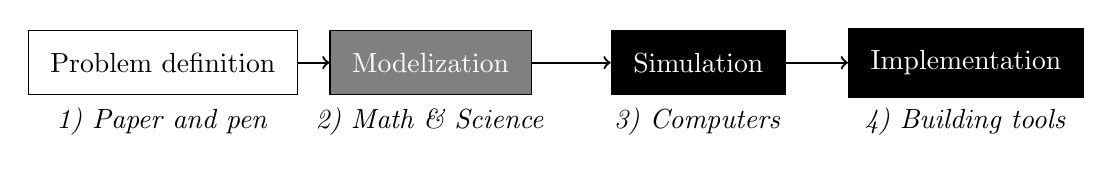
\begin{tikzpicture}

%\pgfdeclareimage{bulb}{assets/light-bulb}

\tikzmath{
	\x = 3.4;
    \sx = \x + \x;
    \ssx = \sx + \x;
    \y = -0.75;
}

\node[draw,inner sep=8pt] (prob) at (0,0) {Problem definition};
\node[draw,inner sep=8pt,fill=gray,text=white] (mod) at (\x,0) {Modelization};
\node[draw,inner sep=8pt,fill=black,text=white] (sim) at (\sx,0) {Simulation};
\node[draw,inner sep=8pt,fill=black,text=white] (impl) at (\ssx,0) {Implementation};

\draw[->,draw=black,thick] (prob) to (mod);
\draw[->,draw=black,thick] (mod) to (sim);
\draw[->,draw=black,thick] (sim) to (impl);

%\node {\pgfbox[center,bottom]{\pgfuseimage{bulb}}};

\node at (0, \y) {\textit{1) Paper and pen}};
\node at (\x, \y) {\textit{2) Math \& Science}};
\node at (\sx, \y) {\textit{3) Computers}};
\node at (\ssx, \y) {\textit{4) Building tools}};

\end{tikzpicture}

%
% If not, use
%\picplace{5cm}{2cm} % Give the correct figure height and width in cm
%
\caption{Illustration of the different phases in the scientific approach to solve a problem.
Each one of them is executed with different tools and require different skills.}
\label{fig:sciappr}
\end{figure}
%

This way of doing things (visualized in figure \ref{fig:sciappr})
is called: \textit{scientific approach} and is at the very core
of what scientists, mathematicians and engineers do every day. So let's start
with the first step: what problem do we want to solve?

\begin{proposition}[Problem definition]
\label{prop:opinionproblem}
Consider the community of people inside a city. The city council has set a goal to reduce
the amount of cars, plastic and pollution on the whole urban area with the intention of
promoting sustainability, green resources, and renewable energies.

The city administration, however, does not have much money to enforce the new green policies
it wants, so it has to rely on the citizens to try to adopt a more green and sustainable life
in complete autonomy. So they have hired us, a group of scientists, to find a solution to
this problem.
\end{proposition}

Proposition \ref{prop:opinionproblem} seems quite tough right? We are now scientists and we
have been given the job to try to convince the inhabitants of a whole town to change their
daily lives and habits to be more green and sustainable (using less plastic, riding bikes instead of
cars, trash fewer objects, etc.). How are we going to do that?
For starters, no panic! We have an approach to follow, so let's use the method pictured in figure
\ref{fig:sciappr} to solve our problem.\\

Where are we in that diagram? We have passed the first stage as we now know what problem we must focus
on. So now it is time to think about the solution and we do that by using Mathematics and Science. What we
want to study is basically a population made of different individuals: men, women and children.
The city council wants us to find a way to persuade the citizens to change their lifestyle. Changing
a person's behavior or habits means to change their opinion on specific matters. No, we are not talking
about \textit{Inception}\footnote{A sci-fi/thriller movie released in 2010 where a group
of people attempt to plant an idea inside a man's mind by violating his dreams. 
If you haven't see
it, you should because it's pretty cool: \url{https://www.imdb.com/title/tt1375666/}.}, we want to
use less drastic/invasive (and more legal) strategies. One common way of doing this is by
running an \textit{advertising campaign} with tv spots and street cartboards to promote
the concepts we want. However remember that we don't have mush money, so we cannot run these ads all
over town as it would be too expensive: we have a limited budget, which means we can only run small
local campaigns in blocks or areas of the city. Would this strategy suffice?\\

From different social studies, like mentioned by Flache et al. \cite{flache-opinion},
it has emerged that people change their opinion also in relation to
the community where they live. Try to think about one time where your opinion about something shifted,
and try to recall what caused that change: most likely it was because you met and talked with another
person about that subject and the conversation made you change your mind. All that being said,
of course folks' opinion doesn't vary so quickly with just one interaction, it depends
on which person we meet and what topic we are focusing on. Also, people are very different: some
change opinion quite easily, while others are much more stubborn.

However, here's the most important point, no matter how easily a person's opinion change, what matters
is that it can actually change and the change is caused by the opinions of other individuals. Is like
if opinions were contagious to a certain extent. So, since we cannot run a town-wide ad campaign, we can
rather do the same but in a few areas of the city to change a few people's mind
about sustainable lifestyle so that they will later influence their neighbors. But how many citizens
do we need to convince to have enough of them so that their influence will spread across the whole town?
Should we run a bigger campaign on a single city block? Or smaller campaigns in more different areas
of town? Or some other strategy?
To answer that question, we are going to use... you guessed it: a CA!\\

To use a CA for our problem, we need to create one, so we must define its properties:

\begin{enumerate}
\item \textbf{What do the cells represent?} A cell represents a single individual (citizen) in the city.
A cell's neighborhood represents the people that live close to that person
(same building, same city block, etc.).
\item \textbf{What is the state of a cell?} Every individual (cell) can be either: \textit{convinced}
($1$, active, black), or \textit{unconvinced} ($0$, inactive, white) about sustainable lifestyle.
\item \textbf{How do we define the state transition function?} The main idea is that a non convinced citizen
would become convinced if there is a sufficient number of his neighbors that are convinced as well.
Of course the opposite applies as well: if a great number of his neighbors is not convinced,
a convinced individual will also turn unconvinced.
\end{enumerate}

We have the basics of our CA, but we need to work more on the transition function. If we read again the
last point in our list above, we can express with simple mathematical expressions what we wrote:

\begin{proposition}[Opinion shift CA transition function]
\label{prop:opicatrans}
Given a cell $y_{i,j} \in E$ in our opinion analysis CA, its next state is defined by this
transition function:
\begin{equation}
f(n) =
  \begin{cases}
    0       & \quad n < N^\ast\\
    1       & \quad n \geq N^\ast\\
  \end{cases}
\end{equation}
Where $n = 0 \dots 8$ is the number of active neighbors of $y$, and $N^\ast = 0 \dots 9$ is a threshold
value.
\end{proposition}

As you can see from proposition \ref{prop:opicatrans}, transition function $f$ uses a value $N^\ast$ to
set a point where a citizen changes his mind, this number is quite important:

\begin{definition}[Turning Point]
\label{def:tp}
When the transition function $f$ is defined as in proposition \ref{prop:opicatrans}, then quantity
$N^\ast$ is called: \textit{Turning Point} (TP).
If at least $N^\ast$ neighbors are convinced about
a topic, then a citizen would turn or remain convinced too, while if the number of convinced neighbors
is below that number, then a citizen would turn or remain unconvinced.
\end{definition}

Let's talk a bit more about the TP.

\begin{proposition}[Meaning of the Turning Point]
The TP, as per definition \ref{def:tp}, is a quantity and a parameter of our model which,
depending on its value, can describe different important behaviors of individuals in the population,
as shown in table \ref{tab:meaningn}.
\end{proposition}

%
% Table
%
\begin{table}[!t]
\centering
\caption{Showing the meaning of TP $N^\ast$ in relation to the behavior of individuals
in the population.}
\label{tab:meaningn}
%
% Follow this input for your own table layout
%
\begin{tabular}{p{0.15\textwidth}p{0.25\textwidth}p{0.5\textwidth}}
\hline\noalign{\smallskip}
Range of $N^\ast$ & Meaning & Description \\
\noalign{\smallskip}\svhline\noalign{\smallskip}
$N^\ast = 0$ & Stubbornly convinced & No matter what his
neighbors think, this person will never ever turn unconvinced.\\
$1 \leq N^\ast \leq 2$ & Easy to convince  & Such a person does not
require many neighbors to change his feelings about the topic.\\
$3 \leq N^\ast \leq 5$ & Reasonable/average & It takes a fair
intermediate amount of neighbors to make him change his mind.\\
$6 \leq N^\ast \leq 8$ & Hard to convince & A fairly high amount of
neighbors is required to convince people like this to shift their opinion.\\
$N^\ast = 9$ & Stubbornly unconvinced & No matter what his
neighborhood thinks about the topic, this citizen would never ever turn convinced about it.\\
\noalign{\smallskip}\hline\noalign{\smallskip}
\end{tabular}
\end{table}
%

So, we can choose to create a CA where all the citizens have a certain value of $N^\ast$, and
we could create different scenarios where citizens are easy to convince or hard to do so.
By inspecting the evolution of the CA, we would know how to create small ad campaigns to ensure
that the highest possible number of citizens can become convinced about sustainable lifestyle.

\subsection{Building the automaton}
Now it's time to jump on stage 3 of figure \ref{fig:sciappr}. We can finally start coding to
create this new CA. Of course we are not going to reinvent the wheel and start from scratch: we
have already created an automaton: CGL, so let's start from that project and modify a few things.
It turns out that not much code needs to be written to edit CGL and turn it in into this new
automaton we want to build now.

\begin{enumerate}
\item Go to the folder containing our project directory \texttt{cellautom}.
\item Duplicate directory \texttt{cellautom} and name the clone: \texttt{opinionca}.
\item From now on, work inside \texttt{opinionca}.
\end{enumerate}

We have basically duplicated CGL and prepared a copy of it we will edit. In fact, now we must
make a few adjustments in code to develop a different automaton.

\begin{programcode}{ca.js (snippet)}
Open \texttt{ca.js} and spot function \texttt{calculateState}. Remove the content of the
function and place this code instead.
\begin{codeh1}{1}{9}
function calculateState(state, neighSum) {
  const N = 3; // Turning Point

  if (neighSum > N) {
    return 1;
  } else {
    return 0;
  }
}
\end{codeh1}
\end{programcode}

We have re-written function \texttt{calculateState}, which is, basically, the state
transition function in code. Now we have a completely different set of rules and this is
not CGL anymore. We have completed coding the first prototype of an
\textit{threshold-based opinion automaton}\footnote{The complex name indicates the way
our automaton describes the opinion of individuals in a population: by using a threshold that we
have called \textit{Turning Point}. In this automaton, a cell changes state when the number
of active neighbors exceeds a certain threshold, that is: $N^\ast$.}.

\subsection{Running simulations}
In our plan (visualized by figure \ref{fig:sciappr}), we are still in stage 3. We have just built
a simulation program (our web application) which runs a CA to describe opinion change in a
city. Now what we need to do is to use this simulator and run it to produce some data. The data
we collect is going to give us the information we want to learn new things that we can use to reach
our goal (as per proposition \ref{prop:opinionproblem}). How do we use the CA? As we have learnt
so far, we need to set different initial conditions and see how the CA evolves.

\begin{proposition}[Simulation strategy]
\label{prop:simstrat}
Given our objective in proposition \ref{prop:opinionproblem}, we want to try to run an ad
campaign on a targeted small set of communities in town, to meet the low budget. We want to try
different configurations of \textit{short-range local campaigns} in the city,
and see how the opinion changes with time. We will select the configuration which ensures
maximum coverage as the automaton evolves.
\end{proposition}

What do we mean by running \textit{short-range local campaigns}?

\begin{itemize}
\item \textbf{Short-range:} An ad campaign will involve few people in a precise area of the city.
\item \textbf{Local:} The community which is targeted by an ad campaign will be covered 100\%, it
means that there will be no individual in the community who won't be exposed to the campaign.
\end{itemize}

The two points explain that, basically, in our CA,
a targeted community will be a \textbf{small} surface (short-range) of black cells
\textbf{without white holes} inside it (local). If we follow this simulation strategy as per proposition
\ref{prop:simstrat}, we basically need to experiment with some initial conditions consisting of small
black areas located on the city territory. We need to find the best arrangement of black areas that
ensures the CA will evolve to a configuration with the highest amount of black cells in the end.
So this is what we are going to do:

\begin{enumerate}
\item Set an initial configuration for the CA, with some small black area located in
different parts of the grid.
\item Make the CA evolve until a final or recurrent configuration is reached.
\item Take note of the percentage of black cells in the automaton after its evolution. We will call this
measure: \textit{coverage ratio} or \textit{coverage percentage}.
\item Start again trying a different configuration.
\end{enumerate}

At the end, we will compare all the coverage percentages, and we will pick the initial condition
associated to the highest coverage percentage. That initial configuration will be the best
advertising strategy to reach our objective and solve the problem.

\subsubsection{Experimenting a little}
The only requirement is to use small black areas when setting the initial configuration, so
we can have many different possibilities. To avoid making many attempts, we can try to perform
a few simple experiments to see how the CA we built behaves, so that later we can try some more
specific initial conditions and save a lot of time.

The first thing we wanna do, is changing the size of our automaton.

\begin{programcode}{ca.js (snippet)}
In \texttt{ca.js}, at the beginning of the module, change the size of the CA to 40x40.
\begin{code}
const rowsnum = 40;
const colsnum = 40;
\end{code}
\end{programcode}

We need a big automaton to describe a city, we cannot use a 9x9. Feel free to use a larger grid if
you want, however we recommend to have a minimum size of 40x40.\\

We will need to create small surfaces of active cells, we think that drawing small rectangles
is probably the best option to model a local city block or set of apartments. 
From now on, we will refer to a rectangle of black (active) cells as a \textit{block} of cells.
And we are going to draw many blocks. Instead of manually creating a block by filling the
\texttt{initConfig} constant array, which can be tedious, we want to create a function
to which we provide the top-left corner cell and the bottom-right corner cell's coordinates, and it
will push all the cells inside these boundaries into the array \texttt{initConfig}.

\begin{programcode}{ca.js (snippet)}
In our Javascript module, add this function at the beginning, after the constants and variables.
\begin{codeh2}{0}{2}{4}{8}
const initConfig = [];

let t = 0; // Cycles (time)

function setInitialCondition() {
    // In this function, we will populate array 'initConfig'
}
\end{codeh2}
Also note that we have removed any initial value in array \texttt{initConfig}, which now is set
to an empty value at the beginning.

Then, go at the bottom of the module, and insert the highlighted line.
\begin{codeh1}{8}{10}
window.addEventListener("load", function () {
  if (rowsnum < 9 || colsnum < 9) {
    throw new Error("The CA must be at least 9x9.");
  }
  if (cellsize < 4) {
    throw new Error("Cells are too small. A cell must be at least 4px!");
  }

  setInitialCondition();
  create();
  initializeGrid();
  initializeButton();
  updateCycleText();
});
\end{codeh1}
\end{programcode}

What we have done is adding another step in our CA initialization sequence. As you can see from
the last snippet of code, we invoke function \texttt{setInitialCondition} right before everything
else. This function, which we will implement in a moment, will populate array \texttt{initConfig}
in a smarter way.

The next thing we need is a quick way to draw a rectangle as we mentioned before. We will create
a function to accomplish that.

\begin{programcode}{ca.js (snippet)}
Add this function in the Javascript module right after function \texttt{setInitialCondition}.
\begin{code}
function rect(i1, j1, i2, j2) {
  // Must: 0 < i1 < i2 < rowsnum AND 0 < j1 < j2 < colsnum
  for (let i = i1; i <= i2; i++) {
    for (let j = j1; j <= j2; j++) {
      initConfig.push(i + ":" + j);
    }
  }
}
\end{code}
\end{programcode}

Function \texttt{rect} will push inside \texttt{initConfig} all the cells that fall inside the
boundaries defined by point \texttt{i1:j1} and \texttt{i2:j2}. The code is quite simple, we have
the usual double scanning of the cells of the automaton; however this time we scan the rows between
\texttt{i1} and \texttt{i2} and the columns between \texttt{j1} and \texttt{j2}, instead of
spanning the whole grid. Also notice the comment: it clarifies that the two cell coordinates
passed as input must respect some conditions: basically the two set of coordinates must define
two cells inside the grid and that cell \texttt{i2:j2} must be place below and on the right
of \texttt{i1:j1}.
Let's see this new tool in action and let's draw a square block in the automaton.

\begin{programcode}{ca.js (snippet)}
Remove the comment inside function \texttt{setInitialCondition} and
call function \texttt{rect}.
\begin{codeh1}{1}{3}
function setInitialCondition() {
  rect(3, 3, 5, 5); // 3x3
}
\end{codeh1}
\end{programcode}

If you save and refresh, you will see that a black square has been set as initial condition,
and that this block starts from cell \texttt{3:3} until cell \texttt{6:6} (3x3).
The size of the drawn rectangle is: \texttt{(i2-i1+1):(j2-j1+1)}.

We want to experiment a little and see what happens to square blocks of different sizes when
the CA evolves. So let's draw a few more blocks of different dimension and let's draw some
conclusions.

\begin{programcode}{ca.js (snippet)}
Add more calls to function \texttt{rect} inside function \texttt{setInitialCondition}.
\begin{codeh1}{1}{8}
function setInitialCondition() {
  rect(3, 3, 5, 5); // 3x3
  rect(3, 15, 6, 18); // 4x4
  rect(3, 30, 7, 34); // 5x5
  rect(20, 3, 25, 8); // 6x6
  rect(20, 15, 26, 21); // 7x7
  rect(20, 30, 27, 37); // 8x8
}
\end{codeh1}
\end{programcode}

If you refresh the page, you will see our six squares on the grid. Now we go ahead and make the
CA evolve by using the button we developed and see the result after a few cycles (no more than 5
are really needed). What do we see? The 3x3 square has disappeared completely and the other
squares have just slightly changed shapes but they then remained unchanged.
We can draw the first important learning point here:

\begin{proposition}[Minimum size for alive blocks]
\label{prop:minsizedie}
A block of size $W \times H$, whose shortest dimension is lower or equal than 3: $\min(W,H) <= 3$,
disappears as the automaton evolves.
\end{proposition}

Proposition \ref{prop:minsizedie} draws some more generic conclusions on rectangles instead of squares.
But it is of course valid on squares too, in that case the width and height are always the same so
the proposition reads for square blocks smaller than 3x3, as we witnessed.

\begin{problem}
\label{prob:blocksizedie}
Provide evidence that proposition \ref{prop:minsizedie} is correct by using rectangular blocks
of different sizes instead of squares.
\end{problem}

We have our key learning, so what do we make out of it? Is proposition \ref{prop:minsizedie} a good
finding or a bad one? Think a little about it. We want to create a configuration with small blocks
that will hopefully cause the CA to evolve in a way such that these blocks grow in cycles. But
proposition \ref{prop:minsizedie} has just shown that blocks either shrink and stay or shrink and
disappear. Not good unfortunately. So let's pause and reflect: we know the behavior of
\textit{isolated blocks} now, but why does that behavior occur?

Remember our transition function:
an individual turns convinced only if he has at least 3 convinced neighbors.
Inside a block there are two distinct forces that take place:

\begin{itemize}
\item An \textbf{expanding force} exercised by the surface of contiguous black cells which
try to expand their surface.
\item A \textbf{shrinking force} caused by the border of white cells enclosing the block, they
attempt to reduce the size of the block.
\end{itemize}

A block of
black cells 3x3 is apparently not strong enough and is killed by the outer border of white cells
(the shrinking force is stronger).
But when the size increases to 4 or higher, then the black surface is strong enough to keep its state
and is not affected by the white border (the expanding force equals the shrinking one).
It seems like an isolated block will never create an expanding force which exceeds the shrinking one,
therefore isolated blocks cannot solve our problem as they will never grow.

\begin{problem}
\label{prob:highernblockslive}
Prove that when the Turning Point is 4 or higher, $N^\ast \geq 4$, then isolated blocks can grow.
What does it mean? What conclusions do you draw out if this evidence?
\end{problem}

We need to find a different strategy. Our understanding is that, since isolated blocks are not
strong enough to expand, they probably need reinforcement. So instead of considering isolated
blocks, let's use \textit{connected blocks}. We will now make an experiment and draw two blocks
connected by some cells and see what happens. Again, we do not want to write down one cell at a time
inside array \texttt{initConfig}, as we did for blocks;
we want to create a function that
draws a line of connecting cells from one cell to another to save time and be more efficient
in our experiments (so we have a quick way to draw lines). To achieve this we need a little bit
of Geometry.\\

We eventually want to draw a line of cells from one cell to another. Let's forget about
automata for a moment and let's consider a 2D plane, and let's say we want a way to find
all the points $P = (p_x, p_y)$ that lay on
the segment between two points $A = (a_x, a_y)$ and $B = (b_x, b_y)$.
That equation is the following:

\begin{equation}
\label{eq:kinemseg}
\begin{cases}
p_x = (1-k) \cdot a_x + k \cdot b_x\\
p_y = (1-k) \cdot a_y + k \cdot b_y
\end{cases}
k \in [0,1]
\end{equation}

Equations \ref{eq:kinemseg} are called: \textit{segment equations}, and they work 
this way: parameter $k$ is used as a tuner to move the resulting
point $P$ from $A$ to $B$.

\begin{example}[Using the segment equations]
\label{ex:kinemseg}
Let's take two points on the plane: $A = (4,6)$ and $B = (8,2)$. Draw a coordinate system
on a paper (a squared one is handy in this context),
pick up a unit for both axis, and draw the points at their coordinates. Now draw an arrow
connecting $A$ to $B$ making sure the head points to $B$. Equations \ref{eq:kinemseg}
become:
\begin{equation*}
\begin{cases}
p_x = (1-k) \cdot 4 + k \cdot 8\\
p_y = (1-k) \cdot 6 + k \cdot 2
\end{cases}
k \in [0,1]
\end{equation*}
Let's see how this works. We must use parameter $k$ to get all the points on the segment
connecting $A$ and $B$ (remember that $k$ must be in range: $0 \leq k \leq 1$). If we
start with $k=0$, we get: $P = (4,6) = A$. So at the beginning we start from $A$. If we
set $k=1$, we get: $P = (8,2) = B$. So at the end we get $B$. If everything works the way
it should, if we set $k=0.5$, we expect to get the point which lays in the middle of the
connecting segment. In fact, we have that, for $k=\frac{1}{2}$, $P = (6,4)$; if you draw
this point, you will see it actually sits in the middle of the segment.
If we set $k=\frac{1}{4}$, we get $P = (5,5)$.
If we set $k=\frac{3}{4}$, we get $P = (7,3)$.
As you can see, as $k$ approaches $1$ from $0$, we go from $A$ to $B$ on a line.
\end{example}

In example \ref{ex:kinemseg} we had some fun with equations \ref{eq:kinemseg}
and experienced how they work. So now we need to adapt those equations to our automaton.
The problem is that, in our automaton, we have only integer coordinates, not rational
numbers. What we need to do is called: \textit{approximation}. We need to approximate
the results of equartions \ref{eq:kinemseg} to the closest integer number.
To do that, we just need to apply a ceiling function to $p_x$ and $p_y$ so that we get
these equations instead:

\begin{equation}
\label{eq:kinemsegapprox}
\begin{cases}
p_x = \lceil (1-k) \cdot a_x + k \cdot b_x \rceil\\
p_y = \lceil (1-k) \cdot a_y + k \cdot b_y \rceil
\end{cases}
k \in [0,1]
\end{equation}

When we take a number $x \in \mathbb{R}$ and do this: $\lceil x \rceil$, we are calculating
the \textit{ceiling} of that number: we basically approximate $x$ up to the closest integer.

\begin{example}[Understanding numeric ceiling]
If we take $x = 3$, this number is already an integer, so $\lceil x \rceil = \lceil 3 \rceil = 3$.
If we take a rational number like: $x = 3.3$ then we need to pick up the first integer that
comes after that number; that number is $\lceil x \rceil = \lceil 3.3 \rceil = 4$.
Here are a few more examples: $\lceil 0.2 \rceil = 1$, $\lceil 0.001 \rceil = 1$,
$\lceil 0.999 \rceil = 1$, $\lceil 100.1 \rceil = 101$ and $\lceil 5.5 \rceil = 6$.
\end{example}

Now that we have everything we need to draw lines on a squared grid, we can implement
equations \ref{eq:kinemsegapprox} in code.

\begin{programcode}{ca.js (snippet)}
Add this function right after function \texttt{rect}.
\begin{code}
function line(i1, j1, i2, j2) {
  // Must: 0 < i1, i2 < rowsnum AND 0 < j1, j2 < colsnum
  for (let k = 0; k <= 1; k += 0.01) {
    let p1 = (1-k) * i1 + k * i2;
    let p2 = (1-k) * j1 + k * j2;
    p1 = Math.ceil(p1);
    p2 = Math.ceil(p2);
    initConfig.push(p1 + ":" + p2);
  }
}
\end{code}
\end{programcode}

Function \texttt{line} takes 4 arguments: the coordinates of the two cells we want to connect
with a line, that is \texttt{i1:j1} and \texttt{i2:j2}. Note the comment which clearly
describes the acceptable values of the coordinates: this time we just require the coordinates
to be inside the grid size, the cells can be located anywhere in the automaton. Let's try our
new function.

\begin{programcode}{ca.js (snippet)}
Remove the content of function \texttt{setInitialCondition}, and invoke function \texttt{line}
instead.
\begin{codeh1}{1}{3}
function setInitialCondition() {
  line(3, 3, 10, 30);
}
\end{codeh1}
\end{programcode}

If we save and refresh, we will see our line.
So, let's test our theory about connected blocks. Let's now draw two squares and a line connecting
them to see if the number of black cells increases this time.

\begin{programcode}{ca.js (snippet)}
Remove function \texttt{setInitialCondition}'s content again, and add create two blocks and one
line connecting them.
\begin{codeh1}{1}{5}
function setInitialCondition() {
  rect(2, 2, 6, 6); // 3x3
  rect(20, 15, 26, 21); // 7x7
  line(5, 5, 20, 15);
}
\end{codeh1}
\end{programcode}

As you can see, we have created the line to start from the lower-right corner of the top square to
the top-left corner of the bottom one. Let's refresh and see our initial state, now two blocks
are connected via a thin line of cells. If we try to advance by one cycle in the evolution, we
unfortunately see that the line almost immediately disappears and, as we move on with cycles,
the two blocks (which get isolated) will change shape recurrently but will not expand. The line
is not strong enough, we need a thicker line.

\begin{programcode}{ca.js (snippet)}
Add this line of code inside function \texttt{line}.
\begin{codeh1}{8}{10}
function line(i1, j1, i2, j2) {
  // Must: 0 < i1, i2 < rowsnum AND 0 < j1, j2 < colsnum
  for (let k = 0; k <= 1; k += 0.01) {
    let p1 = (1-k) * i1 + k * i2;
    let p2 = (1-k) * j1 + k * j2;
    p1 = Math.ceil(p1);
    p2 = Math.ceil(p2);
    initConfig.push(p1 + ":" + p2);
    initConfig.push(p1 + ":" + (p2+1)); // Thick line
  }
}
\end{codeh1}
\end{programcode}

The line we added will make sure that, every cell \texttt{p1:p2}
we add in the initial configuration, we also add
the cell on its right: \texttt{p1:(p2+1)}. Let's try again in the browser to make the CA evolve
now that the connecting line is evidently thicker than before.
Eureka\footnote{Typical expression mathematicians use when they get at the bottom of
a problem and find a solution. This expression was in fact used by Archimedes
to celebrate a discovery or invention.}! We can finally see that the black surface expands
gradually and, after 18 cycle, the automaton stabilizes onto a final configuration where we have
more black cells than when we started.

\begin{proposition}[Expanding initial configurations]
\label{prop:expinitconfig}
Basing on our experiments, we could assess that the initial configurations that seem to generate
a black surface expanding evolution are those where there are small active connected blocks.
\end{proposition}

\subsubsection{Trying out different initial configurations}
Basing on the findings from our investigations, as per proposition \ref{prop:expinitconfig}, we
now have a strategy. We have discovered that small connected black blocks will expand into wider
black surfaces, which is exactly the effect we want here. So, now the question is about understanding
what specific initial configurations (respecting the characteristics we described in
proposition \ref{prop:expinitconfig}) we should use to get the best result in achieving a solution
to the problem in proposition \ref{prop:opinionproblem}.

\begin{proposition}[Simulation objective]
\label{prop:simobj}
We want to find the initial cnfiguration (or the set of initial configurations, if more can be found)
that cause the opinion-shift automaton to evolve into a configuration with the
highest possible amount of active cells, starting from the fewest possible number of active cells.
\end{proposition}

Let's start with a first attemp: let's create two small blocks at the opposite corners of the city
and let's connect them with a line.

\subsection{Drawing conclusions}
Todo


%%%%%%%%%%%%%%%%%%%%
%%%%%%%%%%%%%%%%%%%%
%%
%% Andrea Tino - 2019
%% Final
%
%% Microsoft Hackathon 2019
%%
%%%%%%%%%%%%%%%%%%%%
%%%%%%%%%%%%%%%%%%%%

\chapter{Final remarks}

We have completed our experience with CA. As you could see, they are beautiful mathematical,
programmable, visual structures that have a variety of different applications. We have experimented
with them by crafting one automaton to study and solve problems in a society; but there are many
more fields where CA can prove to be very useful so we encourage you to keep experimenting more
by creating more automata and check their evolutions.


%
% Andrea Tino
% 2020
%
% =======================================================================
% Creative Commons Attribution-NonCommercial-ShareAlike 4.0 International
% Public License
% =======================================================================
%

\chapter[Solutions]{In-depth learning \& insights}
\label{sec:indepthlearn}

This extra chapter is reserved to more content about topics that were quickly introduced in the book.
Since the main objective is learning by coding, without too much theory in the beginning, in
some cases we had to just introduce some arguments without focusing too much on the theory behind
them. This chapter is about getting that deeper theoretical background if you feel more curious.

Each section covers a specific argument which is referenced in previous chapters in the book.

\input{../packages/YouthCodeAcademy.CntLearningInsights/javascript-modules-1.0.0}


%%%%%%%%%%%%%%%%%%%%
%%%%%%%%%%%%%%%%%%%%
%%
%% Andrea Tino - 2019
%% Solutions
%
%% Programming + Science
%% Cellular Automata
%%
%%%%%%%%%%%%%%%%%%%%
%%%%%%%%%%%%%%%%%%%%

\chapter[Solutions]{Solutions}

\section*{Problems from page \pageref{sec:intro}}

\begin{sol}{prob:evolvetoward111}
\textbf{Find the remaining evolutions}\\
We have already checked, in example \ref{ex:stateled4}, that
$(0,1,0) \overset{f}{\rightarrow} (1,1,1)$, so we need to check the other possible
states different from $(0,0,0)$.
\begin{itemize}
\item If we consider $x_0 = (1,0,0)$, then we have that: $(1,0,0) \rightarrow (1,0,1) \rightarrow (1,1,1)$.
\item If we consider $x_0 = (0,0,1)$, then we have that: $(0,0,1) \rightarrow (0,1,1) \rightarrow (1,1,1)$.
\end{itemize}
The remaining initial configurations are: $(1,1,0)$, $(1,0,1)$, $(0,1,1)$ and $(1,1,1)$. But those are already
known because they are covered by the evolution of the initial configurations we addressed before. For example,
$(1,1,0)$ is the second configuration the CA assumes after $(0,1,0)$.
\end{sol}


\begin{sol}{prob:testcyclic}
\textbf{Period of a cyclic initial condition}\\
In example \ref{ex:stateled3}, we need to start from $x_0 = (1,0,1)$ and calculate the evolution of the automaton.
We have that $x_1 = (0,1,1)$, then $x_2 = (1,1,0)$ and $x_3 = x_ 0 = (1,0,1)$. We got back to the initial
condition after $T=3$ cycles.
\end{sol}

\begin{sol}{prob:changecasize}
\textbf{Change the size of the CA}\\
In \texttt{ca.js}, inside our Javascript module, we have created two contants we can use to set the size of the
automaton. If we change their values, we will get a different size. For example, to have a 20x20 grid,
we just do:
\begin{code}
const rowsnum = 20;
const colsnum = 20;
\end{code}
Or:
\begin{code}
const rowsnum = 20;
const colsnum = 30;
\end{code}
If we want a rectangular automaton.
\end{sol}

\begin{sol}{prob:changeinit}
\textbf{Setting a different initial condition}\\
We have created, inside our Javascript module in \texttt{ca.js}, a constant called: \texttt{initConfig}.
By specifying different cell IDs, we can set a different initial configuration:
\begin{code}
const initConfig = ["3:1", "1:3", "4:4"];
\end{code}
\end{sol}

\begin{sol}{prob:cacolor}
\textbf{Active cells with a different color}\\
We set to black the color of active cells. If you remember, we set this color in our stylesheet
\texttt{style.css}. In there, we need to change the CSS rule for active cells and change the value
of CSS property \texttt{background-color}:
\begin{codeh1}{1}{3}
.cell[data-value="1"] {
  background-color: #f00;
}
\end{codeh1}
In this example, we set it to red.
\end{sol}

\begin{sol}{prob:flowers}
\textbf{Use an image for active cells}\\
To use an image instead of a color to signal that a cell is active, we need to find an image and
make it available in our project:
\begin{enumerate}
  \item In your project folder, create another folder and call it: \texttt{images}.
  \item Search the Internet for an image you like. Try to find a PNG because they will probably have
    a transparent background. If you don't want to spend time doing it, we have an image for you:
    \texttt{flower.png} which you can find under folder \texttt{v2.4.1/images}.
  \item Move the image inside the folder you created in the first step.
\end{enumerate}
Now we need to change the style
of active cells, which means we must edit \texttt{style.css}:
\begin{codeh1}{1}{5}
.cell[data-value="1"] {
  background-image: url("images/flower.png");
  background-position: center;
  background-size: cover;
}
\end{codeh1}
With property \texttt{background-image} we reference the image we want to use (the path is relative to the
CSS file location). Since we want to make sure that the image is placed at the center of the cell, we must use
\texttt{background-position: center}. Finally, we want to ensure that the image exactly takes the size of the
cell and adapts to it, therefore we use \texttt{background-size: cover} which accomplishes exactly that.

If you go ahead and try it (save the stylesheet and refresh the page),
you will see your image popping up where active cells are! Also, if you change the size of a cell,
by changing the value of constant \texttt{cellsize} inside our Javascript module in \texttt{ca.js},
you will see the image will adapt every time.
\end{sol}

\begin{sol}{prob:nextasauto}
\textbf{Automatic evolution of the automaton}\\
Let's start by creating the interface controls: we need to re-label button "Next", and create button "Stop".
In \texttt{index.html}, let's make these modifications:
\begin{codehtmlh1}{1}{4}
<div class="controls">
  <button id="buttonStart">Start</button>
  <button id="buttonStop">Stop</button>
  <span id="cycleText"></span>
</div>
\end{codehtmlh1}
Note that we have both changed the text inside button "Next", as well as changed its ID.
We can now move to \texttt{style.css} to make sure that the styling we had on button "Next" is now
applied to both buttons:
\begin{codecss}
#buttonStart, #buttonStop {
  background-color: #ddd;
  color: #000;
  border: none;
  padding: 5px;
}
#buttonStart:hover, #buttonStop:hover {
  background-color: #ccc;
}
#buttonStart:active, #buttonStop:active {
  background-color: #bbb;
}
\end{codecss}
We have just changed the selectors of the last 3 CSS rules in the file.

The next step is now adding the logic to the buttons, therefore we need to make some changes inside
\texttt{ca.js}. Our strategy is to basically execute the code inside the event handler for button "Next" in
function \texttt{initializeButton} every 1 second; to do that, we need to set an
\texttt{interval}\footnote{In Javascript, an \texttt{interval} is a function that is registered to be
executed every $n \in \mathbb{Q}$ seconds.}. So, let's create a variable at the beginning of the module to
host the interval ID (we will need it to cancel the interval when clicking button "Stop"):
\begin{codeh1}{1}{3}
let t = 0; // Cycles (time)
let int = 0; // CA auto update interval
\end{codeh1}
We then move to function \texttt{initializeButton} and rename it into: \texttt{initializeButtons} as it will now
set the click event listeners to both buttons, not just one. We also modify its logic, so make sure
to re-define the function like this:
\begin{code}
function initializeButtons() {
  // Button "Start"
  let buttonStart = document.getElementById("buttonStart");
  buttonStart.addEventListener("click", function(){
    startAutoUpdate();
  });

  // Button "Stop"
  let buttonStop = document.getElementById("buttonStop");
  buttonStop.addEventListener("click", function(){
    stopAutoUpdate();
  });
  buttonStop.disabled = true;
}
\end{code}
As you can see, we now do something different when the buttons are clicked: we invoke functions: 
\texttt{startAutoUpdate} and \texttt{stopAutoUpdate} that we still need to write. Also note how we
disable the "Stop" button at the beginning, because, when the page loads, we will only allow the user
to start the evolution.
Since we changed the name of the function, we need to update the place where we invoke it, so, down in the module,
make sure to make this modification:
\begin{codeh1}{1}{3}
initializeGrid();
initializeButtons();
updateCycleText();
\end{codeh1}
Time to code the two missing functions we mentioned before, add them below function \texttt{initializeButtons}:
\begin{code}
function startAutoUpdate() {
  int = window.setInterval(function(){
    next();
    updateCycleText();
  }, 1000);

  // Disable the "Start" button
  let buttonStart = document.getElementById("buttonStart");
  buttonStart.disabled = true;
  // Enable the "Stop" button
  let buttonStop = document.getElementById("buttonStop");
  buttonStop.disabled = false;
}

function stopAutoUpdate() {
  window.clearInterval(int);

  // Enable the "Start" button
  let buttonStart = document.getElementById("buttonStart");
  buttonStart.disabled = false;
  // Disable the "Stop" button
  let buttonStop = document.getElementById("buttonStop");
  buttonStop.disabled = true;
}
\end{code}
The first function is executed when button "Start" is pressed, it creates the interval which, after every 1 second,
calls \texttt{next} and \texttt{updateCycleText} (they were called before, once, when clicking button "Next").
The second function stops the interval. Also note how we handle the enabled/disabled states of the buttons to make
sure that, once the auto-update is started, the user cannot start a new one, as well as ensuring that the user
cannot click stop when the evolution has already been interrupted before and never resumed later.
\end{sol}

\begin{sol}{prob:blackcounter}
\textbf{Counting the number of black cells}\\
Let's start from \texttt{index.html} in order to create the new label:
\begin{codehtmlh1}{3}{5}
<div class="controls">
  <button id="buttonNext">Next</button>
  <span id="cycleText"></span>
  <span id="blackCountText"></span>
</div>
\end{codehtmlh1}
We have added a new label with ID \texttt{blackCountText}. Let's now move to \texttt{ca.js} to create the logic for
updating the text inside the label every time the CA changes. We will count the number of black cells by using a
very simple (and slow) approach: every time the automaton advances in a new configuration, we scan all the cells and
count the number of black ones. So, in the module, add this function after function \texttt{updateCycleText}:
\begin{code}
function updateBlackCountText() {
  let count = 0;
  for (let i = 1; i <= rowsnum; i++) {
    for (let j = 1; j <= colsnum; j++) {
      if (get(i, j) === 1) {
          count++;
      }
    }
  }

  let text = document.getElementById("blackCountText");
  text.textContent = "black cells: " + count;
}
\end{code}
As you can see, we go through every cell (border included), and increment variable \texttt{counter} every time
a black cell is encountered. The final part of the function will update the text of the label we added to the
page at the beginning.
Next, we need to call this function, basically in every place where we also call function \texttt{updateCycleText};
that is when the CA is rendered (at the end of the module):
\begin{codeh1}{2}{4}
initializeButton();
updateCycleText();
updateBlackCountText();
\end{codeh1}
And every time the automaton changes (inside function \texttt{initializeButton}):
\begin{codeh1}{2}{4}
next();
updateCycleText();
updateBlackCountText();
\end{codeh1}
As mentioned, this approach makes the application slower because we have to re-scan again all the cells.
We encourage you to find a better approach!
\end{sol}

\begin{sol}{prob:cgl1}
\textbf{Blocks in Conway's Game of Life}\\
We can use the original size (9x9) and start from cell \texttt{3:3}. We must create
an initial condition with two consecutive active cells, and two active cells below them:
\begin{code}
const initConfig = ["3:3", "3:4", "4:3", "4:4"];
\end{code}
When we save and refresh the page, a block appears. If we click \textit{Next} and follow the
evolution, we see that nothing changes. So a \textit{block}, is a static condition
(see definition \ref{def:staticconf}) in CGL.
\end{sol}

\begin{sol}{prob:cgl2}
\textbf{Bee-hives and tubs in Conway's Game of Life}\\
Let's start creating a \textit{bee-hive} first as shown in figure \ref{fig:cglplay}. We can use
the original 9x9 automaton size because this configuration's size is 3x4, so it fits.
We place the first (left-most and top-most) black cell of the configuration in cell \texttt{3:3},
so we write:
\begin{code}
const initConfig = ["3:3", "3:4", "4:2", "4:5", "5:3", "5:4"];
\end{code}
When we refresh the page we see the configuration and as we advance the CA, we can see that
nothing changes. So a bee-hive is a static configuration.

Let's now draw a \textit{tub} as initial configuration.
This shape's size is 3x3 so it fits the original 9x9 CA.
Its first black cell will be placed in position \texttt{3:3}, so we can write:
\begin{code}
const initConfig = ["3:3", "4:2", "4:4", "5:3"];
\end{code}
Let's refresh and make the automaton evolve: again another static configuration.

If we want to draw both a bee-hive and a tub, we need a bigger automaton. The bee-hive
is 3x4 and the tub is 3x3, we also need to leave at least 3 cell separation
(to avoid one figure to affect the other) between the two figures, which means that a
15x15 automaton should be ok. We will draw a bee-hive on the top-left part of the automaton
and a tub in the bottom-right portion:
\begin{code}
const initConfig = ["3:3", "3:4", "4:2", "4:5", "5:3", "5:4", "10:10", "11:9", "11:11", "12:10"];
\end{code}
As we refresh and make the automaton evolve, we see that the two figures remain there, so a
configuration obtained by combining two static configurations is still static.

Let's have some more fun and experiment a bit longer. What happens if the two static figures
are placed too close to each other? If we try to move the tub very close to the bee-hive like this:
\begin{code}
const initConfig = ["3:3", "3:4", "4:2", "4:5", "5:3", "5:4", "5:6", "6:5", "6:7", "7:6"];
\end{code}
We can see, as we refresh the page and let the CA evolve, that the two figures start changing.
That's because each cell reacts to a neighborhood of radius 1, since one figure's cells are
in the other's cells' neighborhoods, a different evolution happens. In this case the initial configuration
we just created leads to a final configuration which is a bee-hive.
\end{sol}

\begin{sol}{prob:cgl3}
\textbf{Blinkers in Conway's Game of Life}\\
In the original automaton (9x9), we can draw an horizontal \textit{blinker}:
\begin{code}
const initConfig = ["5:5", "5:6", "5:7"];
\end{code}
Or a vertical one:
\begin{code}
const initConfig = ["5:5", "6:5", "7:5"];
\end{code}
In both cases, as we make the automaton evolve, we see that the two initial configurations are
cyclic because we get back to them after two cycles (period $T=2$).
\end{sol}

\begin{sol}{prob:cgl4}
\textbf{Toads and beacons in Conway's Game of Life}\\
Let's first draw a \textit{toad} as shown in figure \ref{fig:cglplay};
this figure takes a 2x4 rectangle, so our original automaton (9x9)
is ok to contain it. We set the first black cell to be \texttt{5:5}:
\begin{code}
const initConfig = ["5:5", "5:6", "5:7", "6:4", "6:5", "6:6"];
\end{code}
As we make this CA evolve, we see a cyclic configuration with period $T=2$
(as it repeats after two cycles).

As for the \textit{beacon}, figure \ref{fig:cglplay} provides us its size: 4x4, which fits
our original CA, so we don't need to change its size. If we set \texttt{3:3} to be the first black
cell of this configuration, we have:
\begin{code}
const initConfig = ["3:3", "3:4", "4:3", "4:4", "5:5", "5:6", "6:5", "6:6"];
\end{code}
Again, trying the evolution, we can see that this is also a recurrent configiration with period $T=2$.
\end{sol}

\begin{sol}{prob:cgl5}
\textbf{Gliders in Conway's Game of Life}\\
Figure \ref{fig:cglplay} shows how a \textit{glider} should look like.  We take
the first black cell of this configuration to be placed in cell \texttt{3:3}:
\begin{codeh2}{0}{3}{3}{5}
const rowsnum = 30;
const colsnum = 30;
const cellsize = 20; // In px
const initConfig = ["3:3", "4:4", "4:5", "5:3", "5:4"];
\end{codeh2}
As you can see, we also changed the size to 30x30 as requested by the problem.
When we try to make the automaton evolve, we see that the figure sorts of moves towards the bottom-right
part of the grid. Although the shape we see repeats itself, its position changes every time,
so we cannot say this initial configuration is cyclic. This is a configuration where the automaton does
not evolve into a specific final configuration, but keeps changing indefinitely (if it were infinite in size).
In our case, however, because of the border effect, the automaton will eventually turn into a block at cycle
$t=100$ and stay there. So, in our case, the glider condition will lead into a final configuration which is
a block.
\end{sol}

\begin{sol}{prob:cgl6}
\textbf{Spaceships in Conway's Game of Life}\\
In figure \ref{fig:cglplay}, we can see the \textit{spaceship} configuration is the biggest listed.
We set the first black cell of this initial condition to be in cell \texttt{7:7}:
\begin{codeh2}{0}{3}{3}{5}
const rowsnum = 50;
const colsnum = 50;
const cellsize = 20; // In px
const initConfig = ["7:7", "7:8", "8:5", "8:6", "8:8", "8:9", "9:5", "9:6", "9:7", "9:8", "10:6", "10:7"];
\end{codeh2}
We have also changed the automaton's size to 50x50.
As we make the CA evolve, we see that the behavior is the same as in solution \ref{prob:cgl5}: the shape
moves down until reaching the border. If the CA had an infinite size, the shape would move continuously
downward, and the automaton would never reach a final configuration, thus making this initial condition, a
\textit{divergent} one as explained in definition \ref{def:divconf}.
\end{sol}

\begin{sol}{prob:blocksizedie}
\textbf{Vanishing rectangular blocks}\\
Let's draw two rectangles on the automaton as initial conditions by using the utility function we coded:
\begin{codeh1}{1}{5}
function setInitialCondition() {
  rect(3, 3, 5, 20); // 3x18
  rect(27, 33, 37, 35); // 3x11
  rect(25, 10, 35, 15); // 6x11
}
\end{codeh1}
We assume, of course, the size of the automaton to be unchanged (40x40). As we refresh the page and make the 
automaton evolve, we can see that the first two rectangles vanish, while the third stays.
\end{sol}

\begin{sol}{prob:highernblockslive}
\textbf{Growing isolated blocks}\\
Let's change the TP first, in function \texttt{calculateState}:
\begin{codeh1}{1}{3}
function calculateState(state, neighSum) {
  const N = 2; // Turning Point
\end{codeh1}
Now we can move to function \texttt{setInitialCondition} to draw some isolated blocks:
\begin{codeh1}{1}{5}
function setInitialCondition() {
  rect(3, 3, 5, 5); // 3x3
  rect(10, 10, 16, 16); // 7x7
  rect(25, 25, 33, 33); // 9x9
}
\end{codeh1}
As we make the automaton evolve, we see the blocks expanding. This means that, when $N^\ast < 3$, the
expanding force is always higher than the shrinking one; that is because we have set the population to
be easier to convince.
\end{sol}

\begin{sol}{prob:highernblockslive2}
\textbf{Shrinking isolated blocks}\\
Following the same procedure in the solution to problem \ref{prob:highernblockslive}, we change the TP
in function \texttt{calculateState}:
\begin{codeh1}{1}{3}
function calculateState(state, neighSum) {
  const N = 4; // Turning Point
\end{codeh1}
Then we can move to function \texttt{setInitialCondition} and draw the same set of blocks (see 
solution \ref{prob:highernblockslive}).
As we make the automaton evolve, we see the blocks shrinking. This means that, when $N^\ast \geq 3$, the
expanding force is always lower than the shrinking one. The population is, in fact, more stubborn now, and
it takes more effort to convince each individual.
\end{sol}

\begin{sol}{prob:opinionproof1}
\textbf{Alternative block connections}\\
In function \texttt{setInitialCondition}, let's create four rectangles and four lines connecting them along
the border of the automaton:
\begin{codeh1}{1}{14}
function setInitialCondition() {
  rect(3, 3, 6, 6); // 4x4
  rect(3, 35, 6, 38); // 4x4
  rect(35, 3, 38, 6); // 4x4
  rect(35, 35, 38, 38); // 4x4
  line(4, 5, 4, 36);
  line(5, 5, 5, 36);
  line(4, 37, 37, 37);
  line(5, 37, 38, 37);
  line(36, 5, 36, 36);
  line(37, 5, 37, 36);
  line(5, 4, 37, 4);
  line(5, 5, 37, 5);
}
\end{codeh1}
We assume the size of the automaton is unchanged (40x40). As you can see, we needed to create eight lines
because we wanted thick ones (otherwise they would have vanished after one cycle). As we make the
automaton evolve, we see that a desired final condition is reached: all cells enclosed by the four
initial black blocks turned black.
Notice that it takes some time (number of cycles) to reach this configuration though.
\end{sol}





%%
% The back matter contains appendices, bibliographies, indices, glossaries, etc.

\backmatter

\bibliography{bibliography}
\bibliographystyle{plainnat}

%%
\printindex

\end{document}

